\chapter{Procura y construccion del sistema HuMath\textregistered QBee de HuMath Space Systems}   

\noindent En el marco del Proyecto C3, una colaboración interdisciplinaria entre la Universidad EAFIT (Colombia) y la Real Universidad de Tecnología de Estocolmo (KTH, Suecia), se planteó la necesidad de desarrollar un sistema de carga inteligente para un vehículo aéreo no tripulado (UAV) orientado al monitoreo ambiental de la biodiversidad y la salud de los ecosistemas en Colombia. Mientras KTH lideró el diseño estructural y aerodinámico de la plataforma UAV, el equipo de EAFIT asumió la responsabilidad de la procura y construcción de la carga, posteriormente denominada HuMath\textregistered QBee.\\

\noindent El proceso de procura comenzó con la identificación de proveedores de sensores ópticos y electrónica de adquisición de datos con características adecuadas para capturar imágenes multiespectrales en rangos visible y cercano al infrarrojo. El financiamiento para la adquisición de estos componentes fue gestionado a través del proyecto 4DAir, una iniciativa de Minciencias dirigida por la Profesora Elena Montilla Rosero, que permitió asegurar recursos para la compra de cámaras, objetivos, filtros y hardware de control. Asimismo, Saab AB, proporcionó fondos para la fabricación de la estructura de la aeronave y supervisó la gestión administrativa y logística del proyecto.\\

\noindent Inicialmente, se había previsto subcontratar la manufactura de la plataforma a una empresa colombiana especializada; sin embargo, limitaciones tecnológicas y de capacidad obligaron a que el equipo de ingeniería de EAFIT, junto con voluntarios de los programas de Ingeniería Aeronáutica de la Universidad Pontificia Bolivariana y de Ingeniería de la Universidad EAFIT, asumiera la fabricación de la estructura del UAV. Este esfuerzo colaborativo garantizó la integración eficiente entre la plataforma aérea y el sistema de carga HuMath\textregistered QBee.\\

% \noindent La construcción del HuMath\textregistered QBee involucró etapas iterativas de ensamblaje mecánico, integración de sensores y desarrollo de software de control. Primero se diseñaron y fabricaron alojamientos impresos en resina para los sistemas ópticos NIR y VIS, asegurando alineación y modularidad. Posteriormente, se integraron los sensores Alvium 1800 U-501m y U-500c de Allied Vision, junto con sus objetivos y filtros, sobre un chasis impreso en PET-G. Paralelamente, se implementó un script en Python para la adquisición sincronizada de datos multiespectrales y georreferenciación en tiempo real.\\

\noindent Este capítulo describe de forma detallada cada una de las fases de procura y construcción del HuMath\textregistered QBee, destacando las decisiones técnicas, los criterios de selección de componentes y las estrategias de colaboración que hicieron posible la materialización de esta innovadora plataforma de monitoreo ambiental.\\



\section{Construcción de los sistemas ópticos seleccionados para la HuMath\textregistered Bee}

\noindent Los sistemas 6 y 7 integran un sensor, un objetivo y un filtro específicos montados sobre la carcasa impresa (Figura~\ref{fig:exploded_assembly}). Esta configuración facilita la fabricación y el mantenimiento, y permite intercambiar o actualizar componentes de forma independiente.\\

\noindent El sensor NIR Allied Vision Alvium 1800 U‑501m (ON Semi AR0522) comparte tamaño de sensor (2592×1944 px) y paso de píxel (2.2 µm) con su homólogo VIS, pero presenta una respuesta cuántica optimizada en 700–1000 nm, ideal para la adquisición de imagenes en este rango espectral. El objetivo HEO Series de 8 mm f/2.5 se monta directamente sobre la montura S‑Mount y ofrece un AFOV de 29.9°. Con 4 g de masa, cumple el requisito de carga útil y minimiza la transmisión de vibraciones. La montura impresa en resina aloja un filtro paso banda de 850 \SI{}{nm} (CWL) y 50 \SI{}{nm} de ancho de banda, 12.5 mm de diámetro, Hard Coated OD 4.0, encajando sobre el barril y fijándose con un anillo roscado que garantiza la alineación sin sobresalir del perfil de la carcasa.\\

\noindent El sensor VIS Alvium 1800 U‑500c (ON Semi AR0521) mantiene los 2.2 µm de paso de píxel y emplea obturación rolling, reduciendo peso y costo. El objetivo Cr Series de 8.5 mm f/1.3, ruggedized por el fabricante, ofrece gran apertura y resistencia a impactos y vibraciones.. El filtro VIS (UV/IR Cut) M25.5×0.50 bloquea 200–370 nm y 750 – 1100 nm, transmitiendo solo 370–750 nm, e integra directamente una montura compatible para el montaje en el objetivo.\\

\noindent La conectividad micro USB‑B facilita la alimentación y transmisión de datos con la Raspberry Pi 4 (Figura~\ref{fig:sistemas_opticos_componentes}). Además, permiten la integración y control de los sensores a partir de un script en python, lo cual da flexibilidad para diseñar el preprocesamiento y captura de las imágenes de ambos sensores de forma simultanea. Esto permite incluso carga confirguracones ya establecidas o actauliza en tiempo real dichas fongiruaciones relacioandas a paramaetros como, por ejemplo, el tiempo de exposiicón o la ganancia.

    

\begin{figure}[h]
    \centering
    \begin{subfigure}[b]{0.48\linewidth}
        \centering
        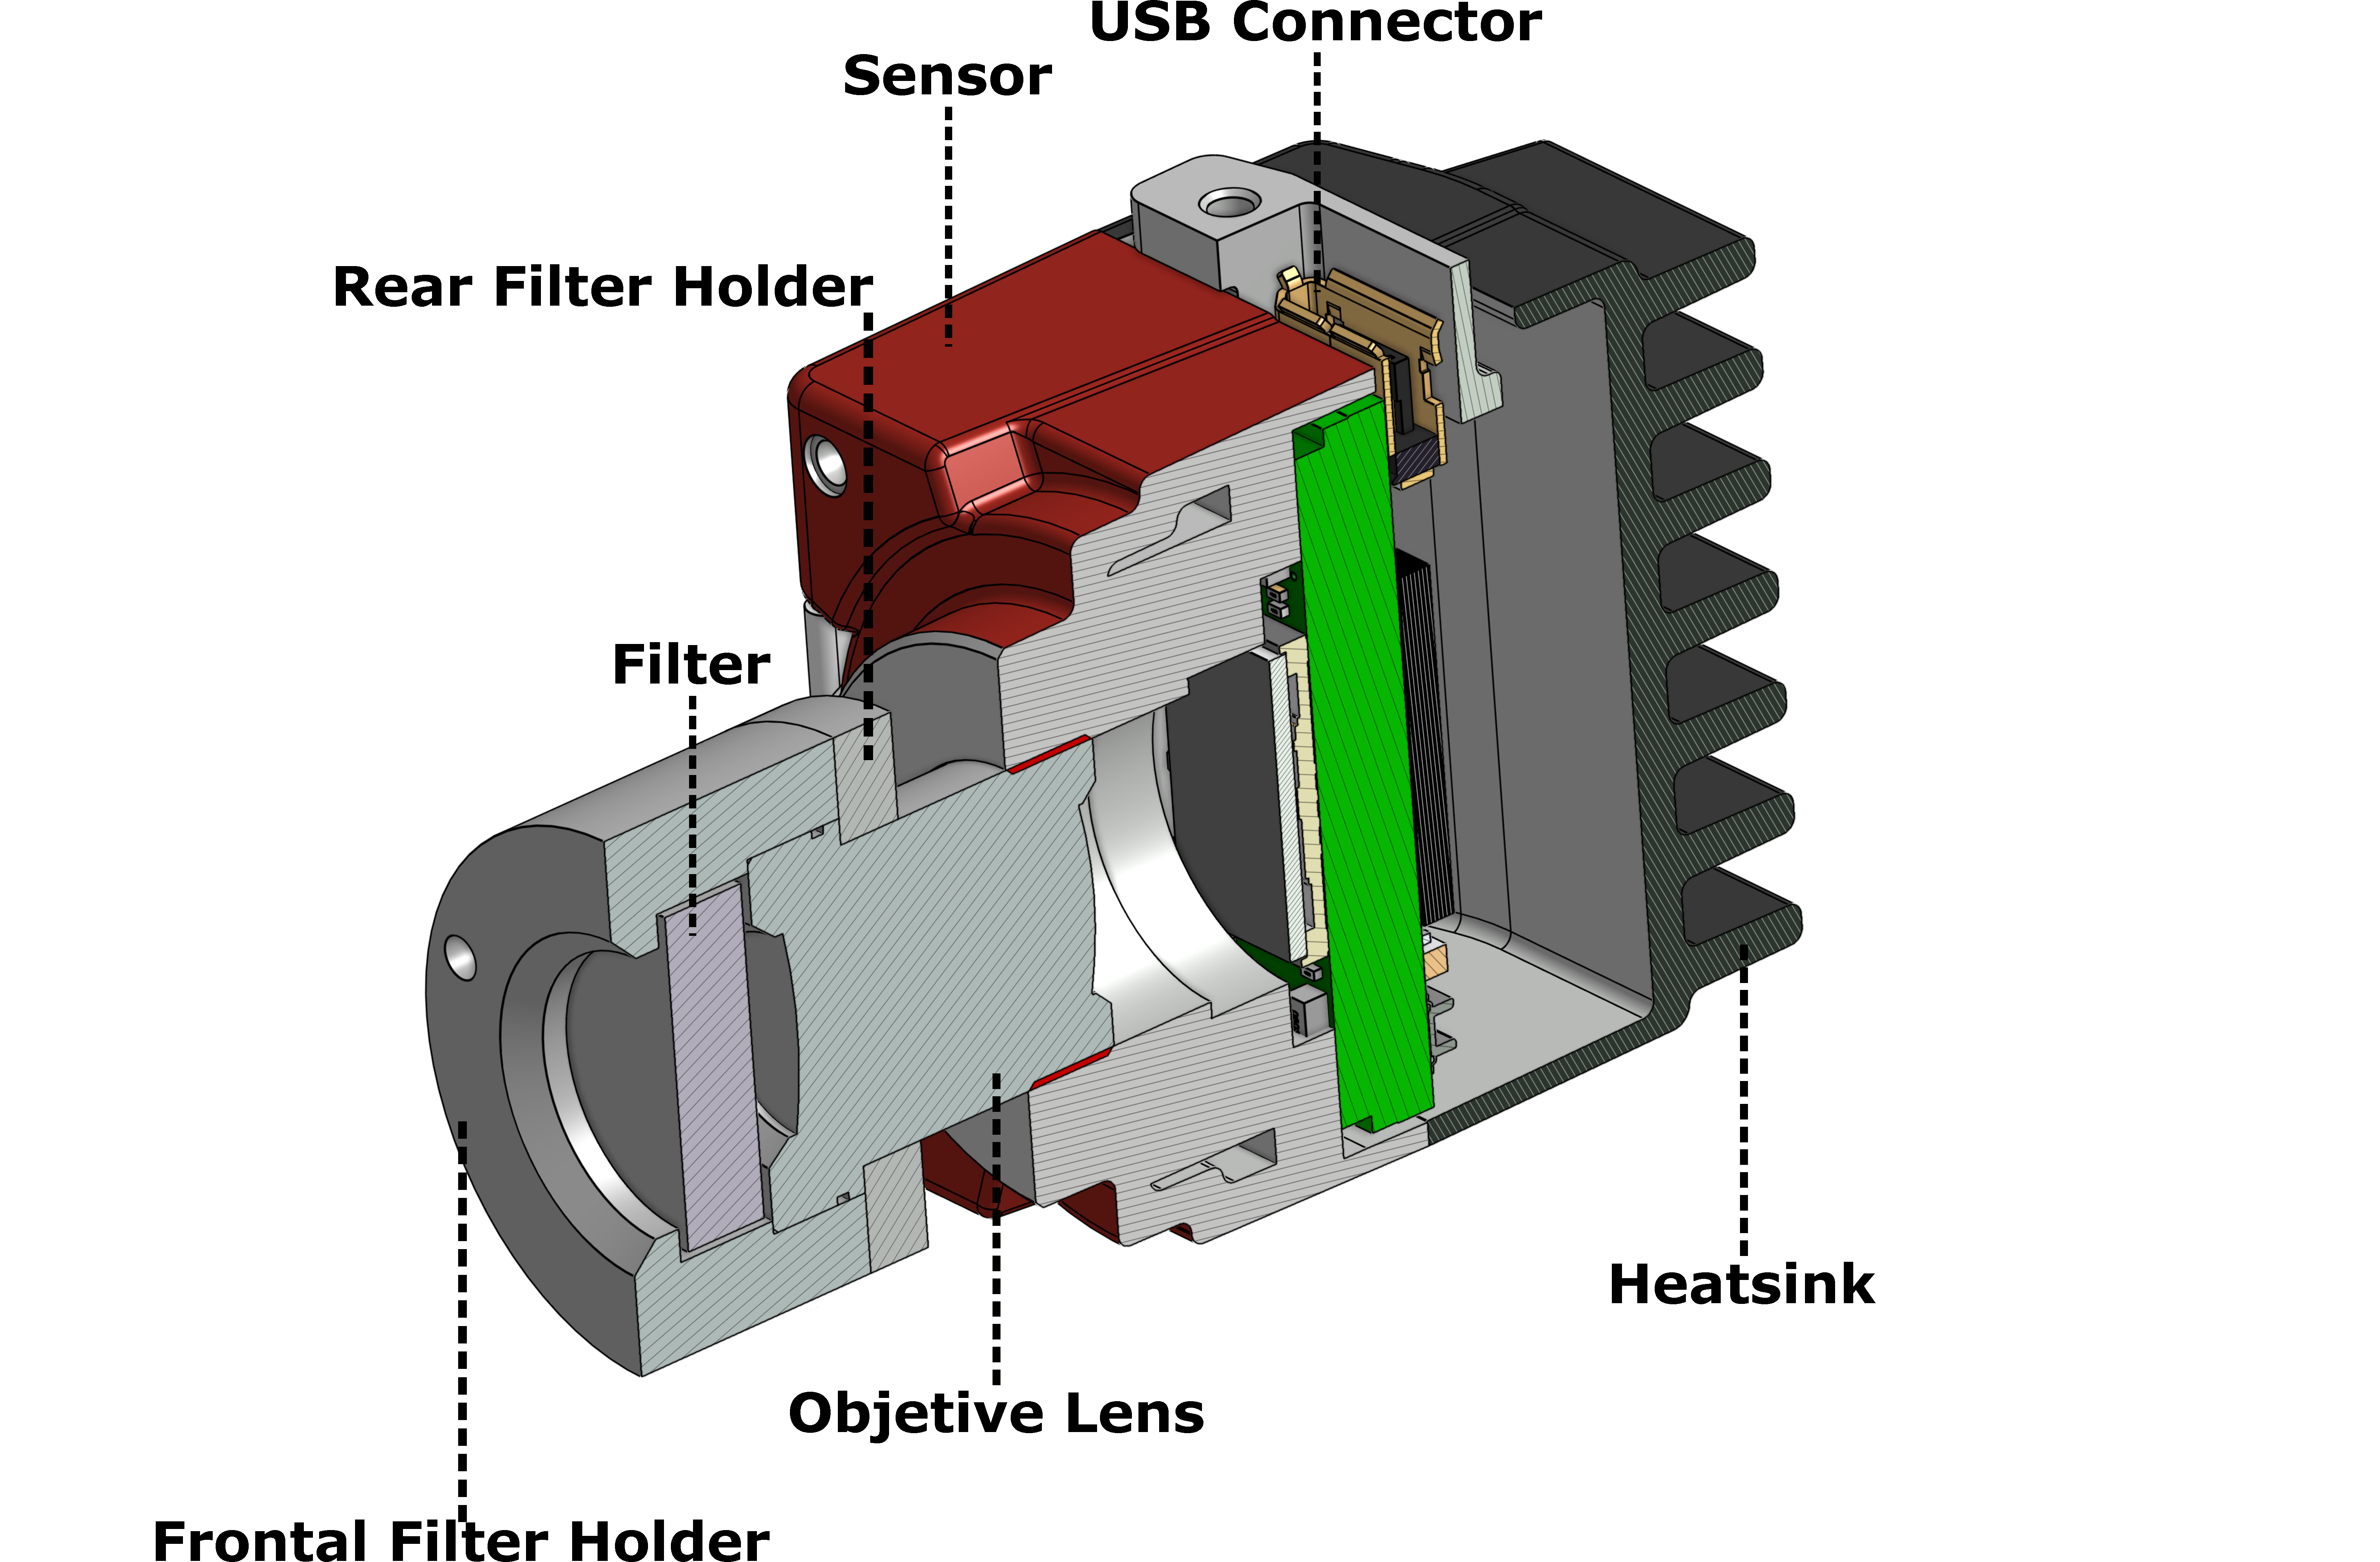
\includegraphics[width=\linewidth]{Figures/C4/NIR1.pdf}
        \caption{Sistema 6 (NIR): montaje del objetivo y filtro. El soporte evita desalineamientos y asegura la óptica en su eje.}
        \label{fig:lens_filter_mount_nir}
    \end{subfigure}
    \hfill
    \begin{subfigure}[b]{0.47\linewidth}
        \centering
        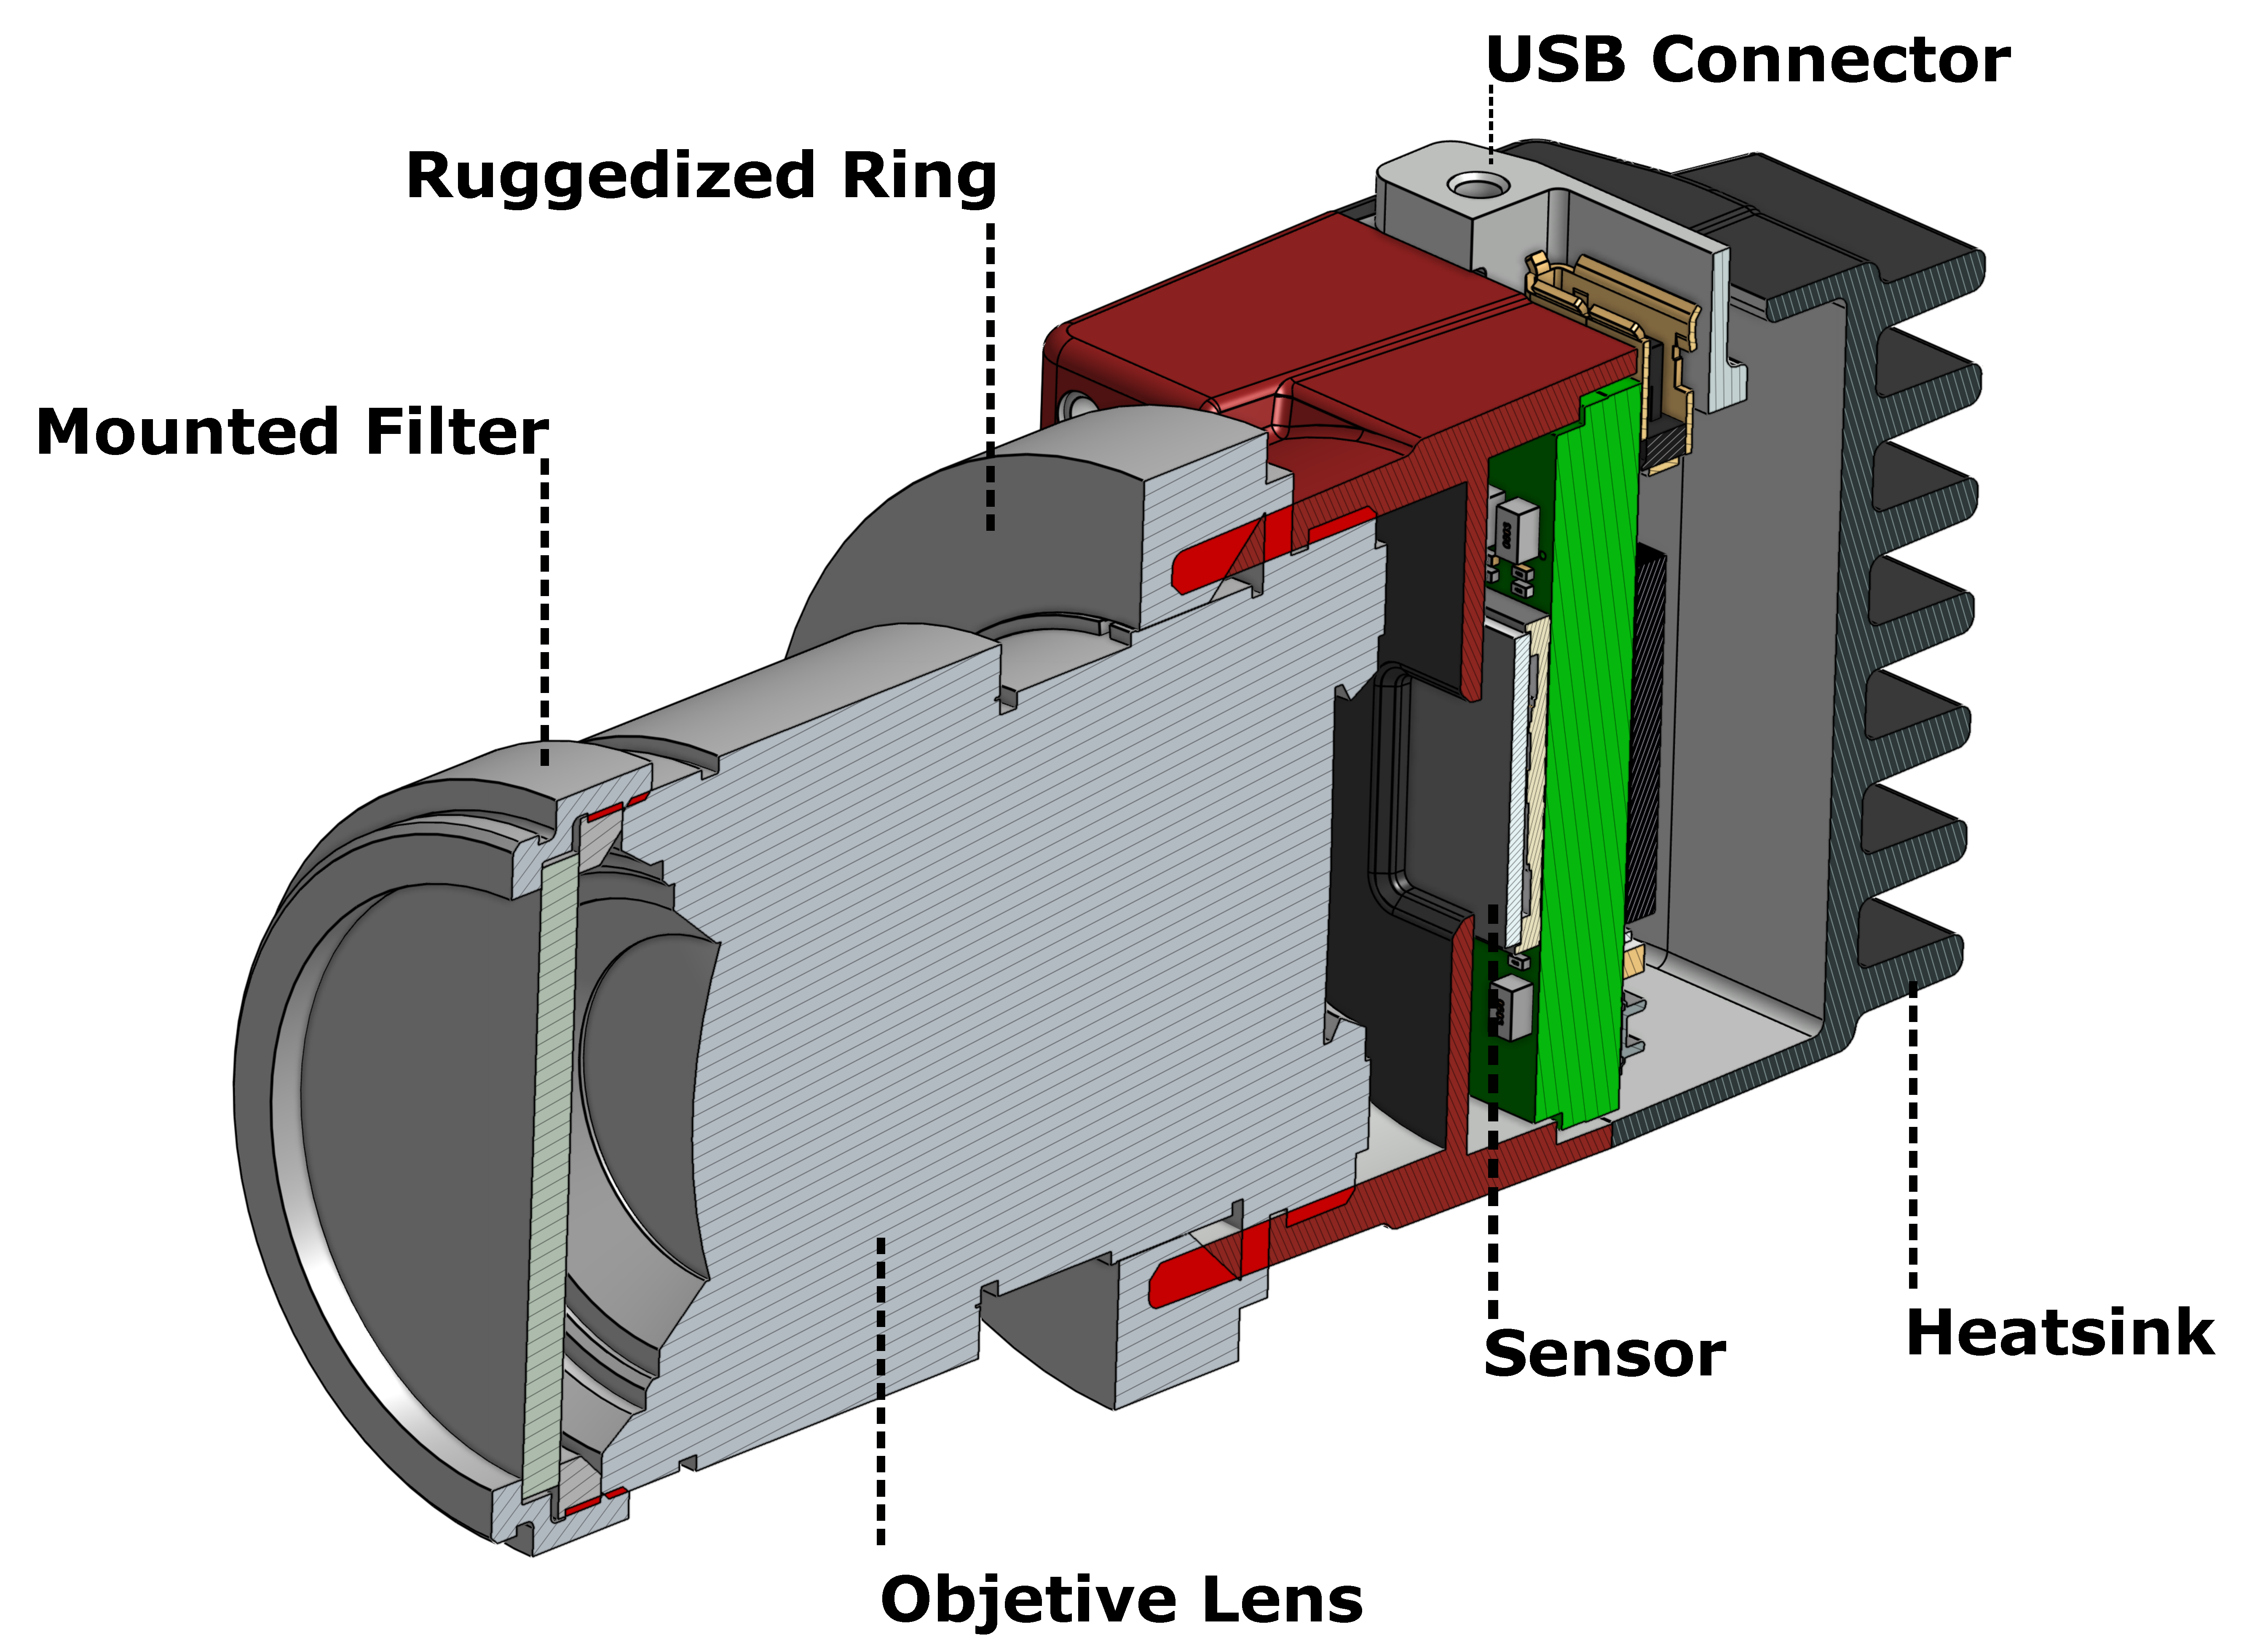
\includegraphics[width=\linewidth]{Figures/C4/VIS1.pdf}
        \caption{Sistema 7 (VIS): conector micro USB‑B para alimentación y datos.}
        \label{fig:micro_usb_vis}
    \end{subfigure}
    \caption{Componentes destacados de los sistemas ópticos seleccionados para el prototipo: NIR (izquierda) y VIS (derecha).}
    \label{fig:sistemas_opticos_componentes}
\end{figure}


  % \subsection{Integración con la plataforma UAV}
  %   % → Describir interfaz mecánica, centro de masas, cableado
  %   %   y sistema de amortiguación de vibraciones.

  % \subsection{Validaciones funcionales de taller}
  %   % → Pruebas de alineamiento, sellado de luz parásita y peso final.
  %   %   Tabla de verificación contra los requisitos de la Sección 1.1.
  \section{Sistema de adquisicion y control de datos}
  \label{sec:script_control_adquisicion}
  
  Con el propósito de automatizar el proceso de captura, procesamiento y almacenamiento de imágenes multiespectrales durante los vuelos o pruebas en banco, se desarrolló un script en lenguaje Python que permite la adquisición simultánea de imágenes en el espectro visible (VIS) y cercano al infrarrojo (NIR), integrando además datos de posicionamiento global (GPS) en tiempo real.
  
  \noindent Este script constituye una adaptación del código de ejemplo provisto por la biblioteca \texttt{vmbpy}, correspondiente al SDK de \textit{Allied Vision}, y fue modificado sustancialmente para incluir manejo multihilo, escritura condicional de video, superposición de información telemétrica, y control por teclado durante la ejecución.
  
  \subsection{Estructura general del script}
  
  El flujo lógico del código se presenta en la Figura~\ref{fig:diagrama_script}, donde se destacan tres etapas fundamentales: (i) la inicialización del entorno y detección de cámaras, (ii) la adquisición concurrente de tramas mediante hilos productores, y (iii) el procesamiento y visualización de las imágenes mediante un hilo consumidor.
  
  \begin{figure}[!h]
      \centering
      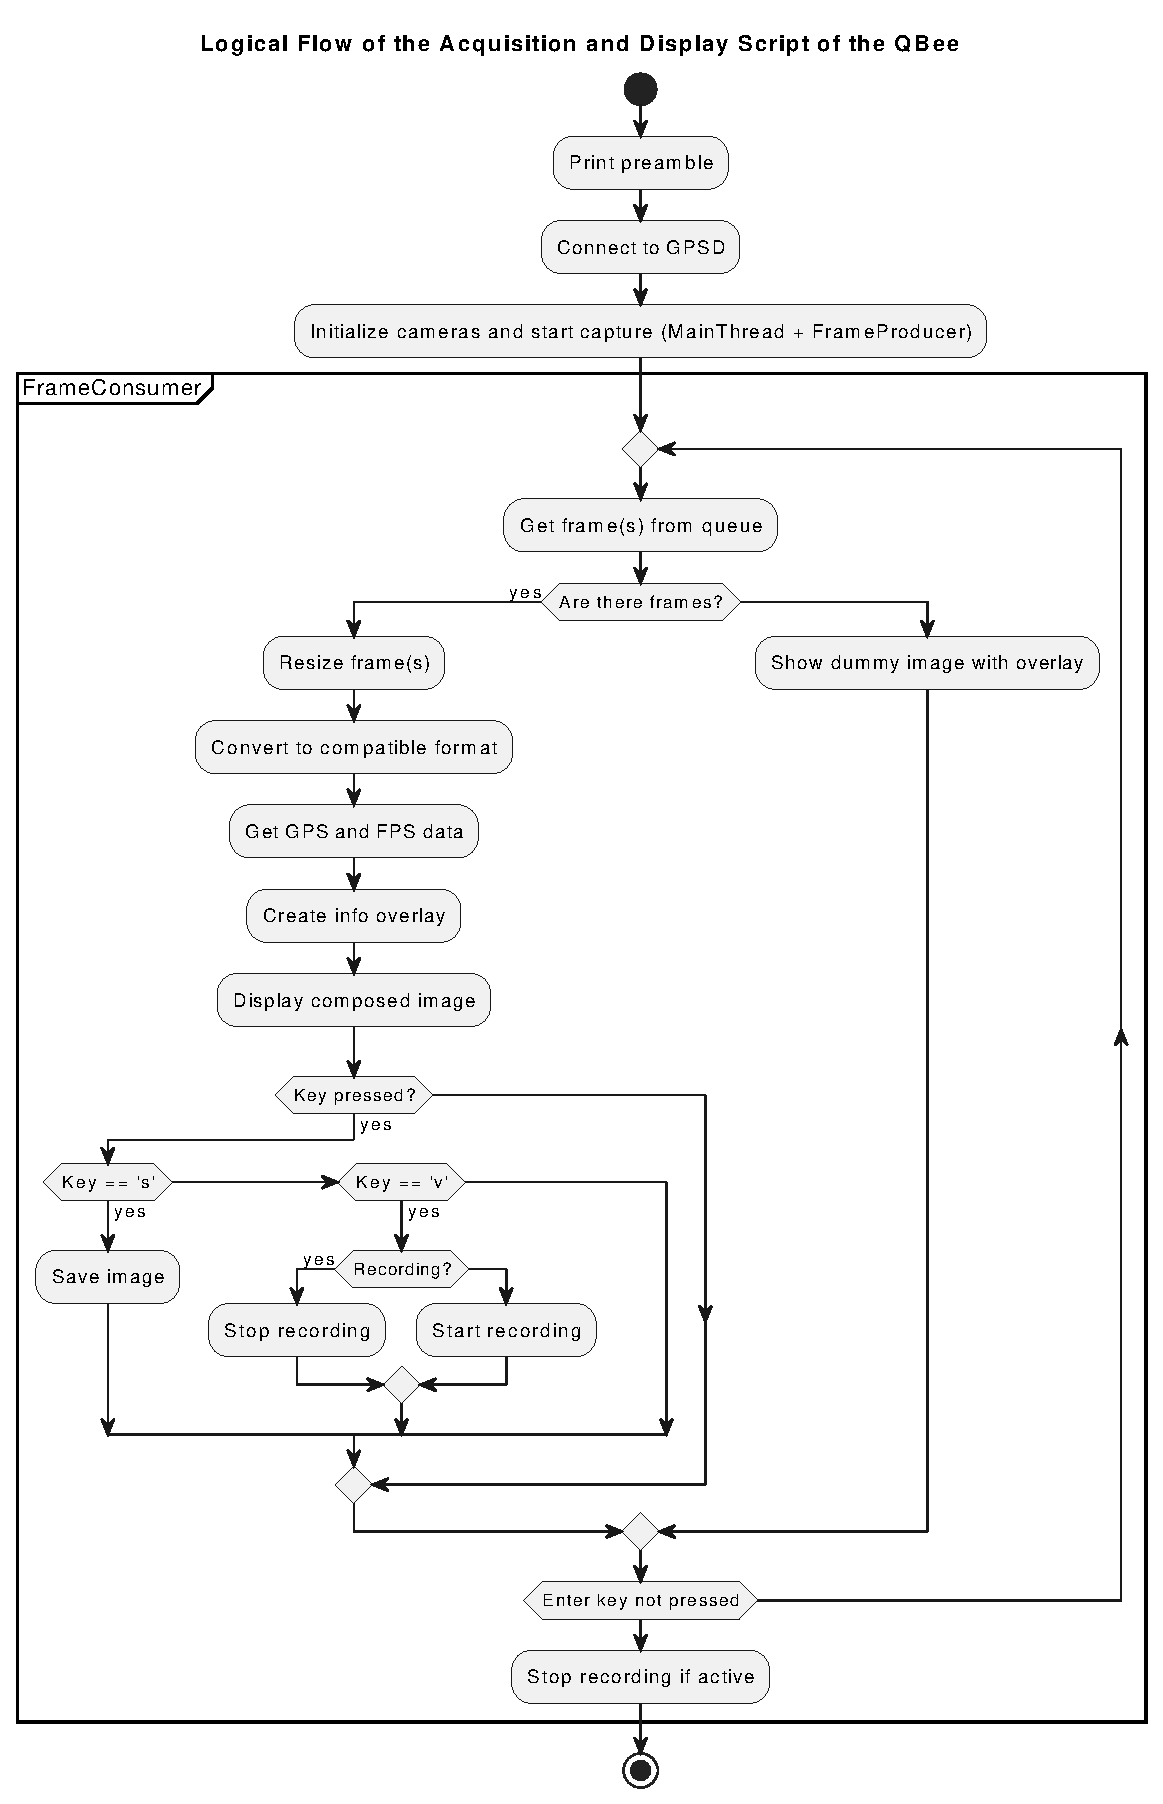
\includegraphics[trim = 0 0 0 1cm, clip, width=1\textwidth]{Figures/C4/OSU_main.pdf}
      \caption{Flujo lógico del script de adquisición y visualización de la QBee. Se integran múltiples cámaras, adquisición en paralelo y procesamiento en tiempo real.}
      \label{fig:diagrama_script}
  \end{figure}
  
  \subsection{Inicialización y adquisición}
  
  Durante la fase de inicialización, se establece una conexión con el servidor local de GPS (\texttt{gpsd}) utilizando la librería homónima. Paralelamente, se instancia la clase \texttt{MainThread}, responsable de detectar automáticamente todas las cámaras conectadas a través del sistema \texttt{VmbSystem}.\\
  
   Cada cámara detectada es asignada a un hilo independiente de la clase \texttt{FrameProducer}, la cual configura parámetros críticos como la resolución de adquisición, formato de pixel (\texttt{Mono8} o \texttt{Bgr8}), y el modo automático de exposición. Estos hilos se encargan de capturar tramas en tiempo real, estimar la tasa de cuadros por segundo (FPS) y encolar las imágenes en una estructura tipo FIFO (\texttt{queue.Queue}) para su posterior procesamiento.
  
  \subsection{Procesamiento, visualización y almacenamiento}
  
  La etapa central del sistema está contenida en la clase \texttt{FrameConsumer}, la cual opera como hilo consumidor. Esta clase realiza múltiples tareas en paralelo: (i) extrae tramas de la cola compartida, (ii) redimensiona las imágenes si la resolución de adquisición no coincide con la esperada (\SI[parse-numbers = false]{2592 \times 1944}{px}), (iii) convierte los formatos de imagen a RGB si es necesario, y (iv) concatena las imágenes capturadas por múltiples cámaras en un único mosaico horizontal.\\
  
  Sobre esta imagen compuesta se genera una barra de información (\textit{overlay}) que incluye los datos georreferenciados en tiempo real (latitud, longitud, altitud, velocidad, ángulo de rumbo y timestamp), además de la tasa de cuadros por segundo estimada para cada cámara. Esta superposición se construye como una matriz adicional que se apila verticalmente a la imagen original.\\
  
  El sistema también permite una interacción directa con el operador mediante teclas específicas:
  \begin{itemize}
      \item \textbf{\texttt{s}}: captura la imagen actual y la guarda en formato \texttt{JPEG}.
      \item \textbf{\texttt{v}}: inicia o detiene la grabación de video en formato \texttt{AVI}, con compresión \texttt{XVID}, a una frecuencia de 20 FPS.
      \item \textbf{\texttt{Enter}}: finaliza la ejecución del script y cierra todas las ventanas.
  \end{itemize}
  
  \subsection{Ejecución automática como servicio de sistema}
  
  Con el fin de garantizar un funcionamiento autónomo y minimizar la intervención del usuario, se diseñó un servicio de sistema en Linux (utilizando \texttt{systemd}) que permite la ejecución automática del script tan pronto como el dispositivo inicia. Este servicio fue instalado y habilitado en el sistema operativo de una Raspberry Pi 4 modelo B equipada con 8 GB de memoria RAM.
  
  Gracias a esta configuración, el sistema conocido como \texttt{QBee} se activa automáticamente al conectar la batería externa a la Raspberry Pi, sin requerir intervención adicional ni acceso al entorno gráfico. Inmediatamente después del arranque, el script inicia la captura de imágenes y comienza a almacenarlas en la memoria interna, lo que resulta particularmente útil para operaciones en campo, donde no es viable iniciar el sistema manualmente.
  
  \subsection{Robustez y tolerancia a fallos}
  
  Durante la ejecución, el sistema cuenta con mecanismos de tolerancia a errores. Por ejemplo, si el buffer de imágenes se encuentra lleno, los hilos productores omiten la encolación de nuevas tramas para evitar bloqueos. Asimismo, si no se detecta ninguna cámara activa, se genera una imagen dummy con un mensaje de advertencia.\\
  
  Las tramas obtenidas se almacenan temporalmente en memoria, lo que permite minimizar la latencia entre adquisición y visualización. La sincronización entre hilos se realiza mediante eventos y bloqueos controlados, garantizando la integridad de los datos entre productores y consumidores.
  
  \subsection{Dependencias y entorno de ejecución}
  
  El script fue ejecutado sobre el sistema operativo Raspberry Pi OS (basado en Debian) en una Raspberry Pi 4 modelo B. Se utilizó Python 3.8 y las siguientes dependencias: \texttt{vmbpy}, \texttt{opencv-python}, \texttt{gpsd-py3}, \texttt{numpy}, \texttt{threading}, \texttt{queue} y \texttt{keyboard}. La visualización se realizó mediante la salida HDMI de la Raspberry, y se requirió establecer la variable de entorno \texttt{DISPLAY=":0"} para habilitar la salida gráfica de OpenCV.

  \subsection{Control remoto del dispositivo \texttt{QBee}}

  Además de su capacidad de operación autónoma en campo, el sistema \texttt{QBee} fue diseñado con funcionalidad de control remoto, permitiendo su supervisión y operación desde dispositivos externos como computadores personales, tabletas o teléfonos móviles. Esta característica extiende significativamente la versatilidad del sistema, facilitando tanto pruebas en laboratorio como operaciones a distancia en entornos de difícil acceso.\\
  
  Existen dos métodos principales para acceder de forma remota a la interfaz gráfica del sistema:
  
  \paragraph{1. Conexión local mediante VNC}
  
  El primer método consiste en conectarse directamente a la Raspberry Pi 4 que ejecuta el sistema \texttt{QBee} mediante el protocolo VNC (\textit{Virtual Network Computing}). Para ello, es necesario que la Raspberry esté conectada a una red Wi-Fi previamente configurada para su conexión automática. Asimismo, el dispositivo de control (computador o móvil) debe encontrarse dentro de la misma red local.\\
  
  Una vez cumplida esta condición, el usuario puede acceder a la interfaz gráfica de la Raspberry Pi introduciendo su dirección IP o una dirección local estática configurada mediante el sistema operativo Raspberry Pi OS. Para completar el acceso, se requiere conocer las credenciales de autenticación (nombre de usuario y contraseña) establecidas previamente en el sistema.
  
  \paragraph{2. Acceso global mediante Raspberry Pi Connect}
  
  El segundo método se basa en el uso de \textit{Raspberry Pi Connect}, un servicio gratuito proporcionado por la fundación Raspberry Pi. Este permite acceder a la interfaz gráfica del sistema desde cualquier lugar con conexión a Internet, sin necesidad de estar dentro de la misma red local.\\
  
  Para habilitar esta funcionalidad, la Raspberry Pi debe estar vinculada a una cuenta en el servicio \textit{Raspberry Pi Connect} y tener acceso a Internet mediante una red Wi-Fi registrada previamente. Una vez registrado el dispositivo, el usuario puede iniciar sesión en el portal de Raspberry Pi y conectarse directamente a su interfaz gráfica a través del navegador.  \\
  
  
  En ambos métodos, el usuario obtiene acceso completo al entorno de escritorio de la Raspberry Pi. Como se ha descrito en las secciones anteriores, el script de adquisición de \texttt{QBee} se ejecuta automáticamente al iniciar el sistema, lo que da lugar a la apertura de una ventana de visualización en tiempo real de las imágenes capturadas.\\
  
  Desde esta interfaz remota, el usuario puede interactuar directamente con el sistema utilizando un teclado virtual o físico para ejecutar acciones de control. Entre las funcionalidades disponibles se encuentran:
  \begin{itemize}
      \item Presionar la tecla \texttt{s} para capturar y guardar una imagen.
      \item Presionar la tecla \texttt{v} para iniciar o detener la grabación de video.
      \item Presionar la tecla \texttt{Enter} para finalizar la ejecución del script.
  \end{itemize}
  
  Esta capacidad de control remoto permite verificar el correcto funcionamiento del sistema en tiempo real, supervisar condiciones de operación, y capturar eventos relevantes sin necesidad de intervención física directa sobre el dispositivo.\\
  
  
  Adicionalmente, el sistema \texttt{QBee} fue configurado para permitir actualizaciones remotas del código fuente del script mediante el sistema de control de versiones \texttt{Git}. El script está vinculado a un repositorio privado alojado en la plataforma \texttt{GitHub}, lo que permite a los usuarios autenticados realizar \textit{pull} de actualizaciones desde cualquier ubicación con acceso remoto al dispositivo. Esta funcionalidad permite una mejora continua del sistema, facilitando la depuración, implementación de nuevas funcionalidades y adaptaciones específicas sin necesidad de acceso físico al hardware.
  

  \section{Construcción e integración del prototipo}
  \subsection{Modelo CAD y ensamblaje mecánico}
    % → FIGURA grande: render CAD explosionado del KBee con leyenda de partes.
    %   Tabla: materiales y masa de cada componente.

    El case del QBee está impreso en PET‑G (tereftalato de polietileno modificado con glicol), un polímero cuya densidad típica ronda 1,317 g/cm³, que combina buena resistencia al impacto (Charpy $\approx$ 4,03 kJ/m²) y alargamiento al rompimiento hasta 15\% en formulaciones estándar. Su módulo de tracción (~4015 MPa) y de flexión (~2987 MPa) aseguran rigidez, mientras que su temperatura de transición vítrea ($\approx$ 76 °C) y rango de fusión (220–260 °C) lo hacen estable en el calor generado por electrónica cercana. Además, presenta excelente durabilidad química y mínima tendencia al \emph{warping}, ideal para piezas de geometría compleja. El peso total del disposito es de 1.810 gramos, cumpliendo así con el requisito de peso impuesto.\\

    \noindent La dimensión externa del case se diseñó para encajar en el bay interno del UAV C3, sin requerir hermeticidad, ya que este estária protegido de las condiciones exteriores. El cierre se logra con tornillos M3 que unen la tapa inferior y el divisor de compartimentos a la carcasa principal. En el interior, cada sistema óptico (6/NIR y 7/VIS) se ancla directamente al sensor mediante cuatro tornillos M3 en sus laterales, asegurando alineación con el eje de vuelo. El sistema 6 (NIR) monta el Alvium 1800 U‑501m (AR0522) + objetivo 8 mm f/2.5 + filtro 850 nm en montura S, todo encapsulado en una montura de resina 3D. El sistema 7 (VIS) agrupa el Alvium 1800 U‑500c (AR0521) + objetivo 8.5 mm f/1.3 ruggedized + filtro VIS UV/IR Cut en rosca M25.5, manteniendo rigidez frente a vibraciones.\\
    
    \noindent La unidad de cómputo y almacenamiento es una Raspberry Pi 4, colocada en un bloque intermedio y alimentada por una powerbank de 20.000 mAh. Este sistema tiene acoplado un hat de GPS, que suministra al sistema de metadatos de fecha, hora UTC, latitud, longitud, altitud y ángulo de elevación, esenciales para la georreferenciación y ortorrestitución de imágenes. Finalmente, el módulo in situ de sensado de contaminantes comparte alimentación de 5 V de la misma batería y ocupa el compartimento trasero de la carcasa, completando la funcionalidad del QBee.\\
    
    

    \begin{figure}[h]
        \centering
        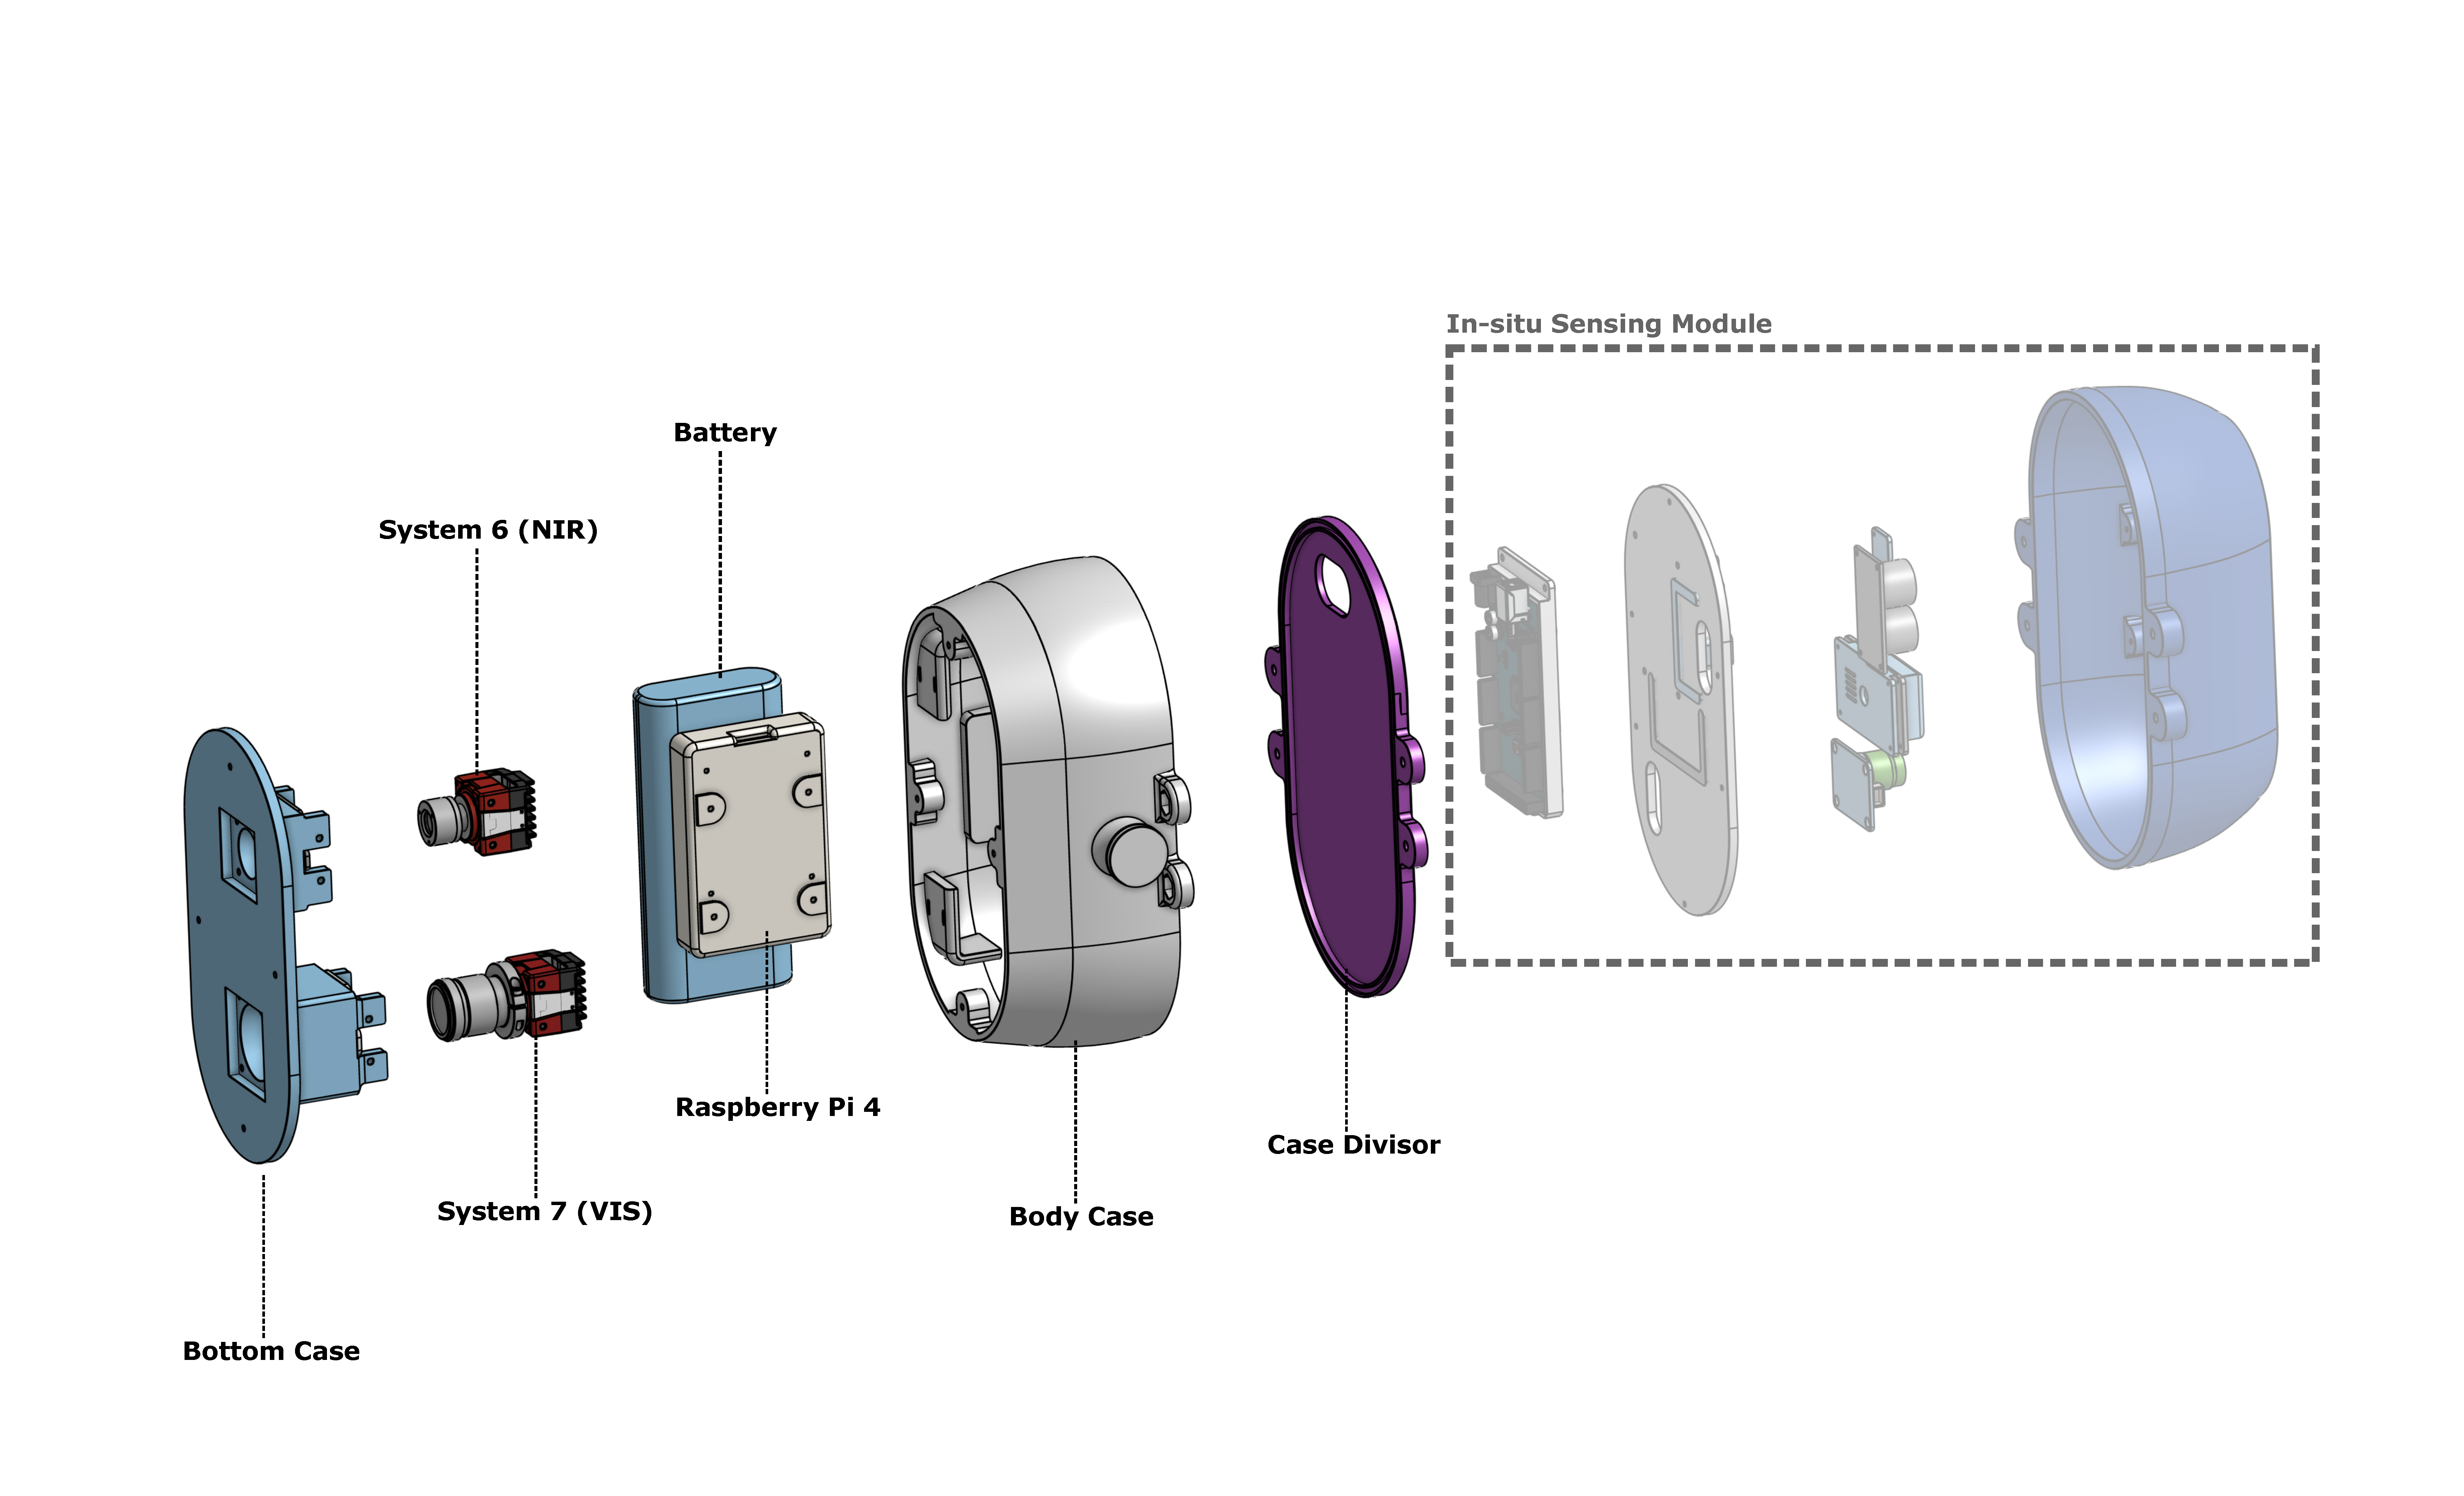
\includegraphics[width=1\linewidth]{Figures/C4/QBee.pdf}
        \caption{Vista explosionada del ensamble completo del QBee, mostrando la carcasa impresa en PET‑G y la disposición de los sistemas 6 (NIR, 8 mm f/2.5) y 7 (VIS, 8.5 mm f/1.8). Este diseño y construcción fue concebido con el apoyo del equipo de manufactura del pryecto C3.}
        \label{fig:exploded_assembly}
    \end{figure}

 

\section{Pruebas de operación}
  
  
  \subsection{Escenarios de prueba}
    Los escenarios de prueba definidos para validar el correcto funcionamiento del sistema \textit{QBee} se clasifican en dos grupos principales: (i) pruebas terrestres en condiciones controladas, y (ii) pruebas en vuelo.

    \subsubsection{Pruebas terrestres}
    
        Antes de cualquier despliegue aéreo, es indispensable realizar pruebas en tierra que permitan validar el sistema en condiciones controladas, sin desplazamiento y sin exposición a ambientes extremos. En este contexto, se define como ambiente extremo cualquier entorno cuya temperatura supere los valores comunes encontrados en las principales ciudades colombianas (\SI{\leq 40}{\celsius}), o que implique lluvia, alta humedad o condiciones de iluminación nocturna.
        
        \noindent Dado que el sistema \textit{QBee} no cuenta con una fuente de iluminación activa, las pruebas se realizan exclusivamente durante el día, aprovechando la luz solar como fuente principal para la adquisición de imágenes multiespectrales.
        
        \noindent El objetivo de estas pruebas es verificar el comportamiento general del sistema en condiciones operativas normales. En particular, se evalúa:
        
        \begin{itemize}
        \item La correcta inicialización automática del script de adquisición al encender el dispositivo.
        \item La funcionalidad de captura de imágenes al presionar la tecla \texttt{s}.
        \item La grabación de video y su detención mediante la tecla \texttt{v}.
        \item La estabilidad del dispositivo al operar durante largos periodos de tiempo.
        \end{itemize}
        
        \noindent Las pruebas se realizaron utilizando dos formas de alimentación:
        \begin{itemize}
        \item \textbf{Fuente directa:} mediante un adaptador USB-C conectado a una toma de corriente convencional.
        \item \textbf{Fuente interna:} a partir de la bater'ia recargable integrada en la carcasa del \textit{QBee}.
        \end{itemize}
        
        \noindent Una de las pruebas más relevantes consisti'o en la captura de una imagen utilizando la tecla \texttt{s}, ya fuera desde un teclado conectado directamente a la Raspberry Pi 4 o mediante acceso remoto. En la Figura~\ref{fig:captura_prueba_remota} se presenta un ejemplo de imagen capturada en estas condiciones, utilizando un tel'efono inteligente para el control remoto del sistema. La prueba confirma el correcto funcionamiento de ambos canales (VIS y NIR), evidenciando que la captura simult'anea se realiza de manera sincronizada, y que el sistema responde adecuadamente a la orden de captura en tiempo real.
        
        \begin{figure}[h]
        \centering
        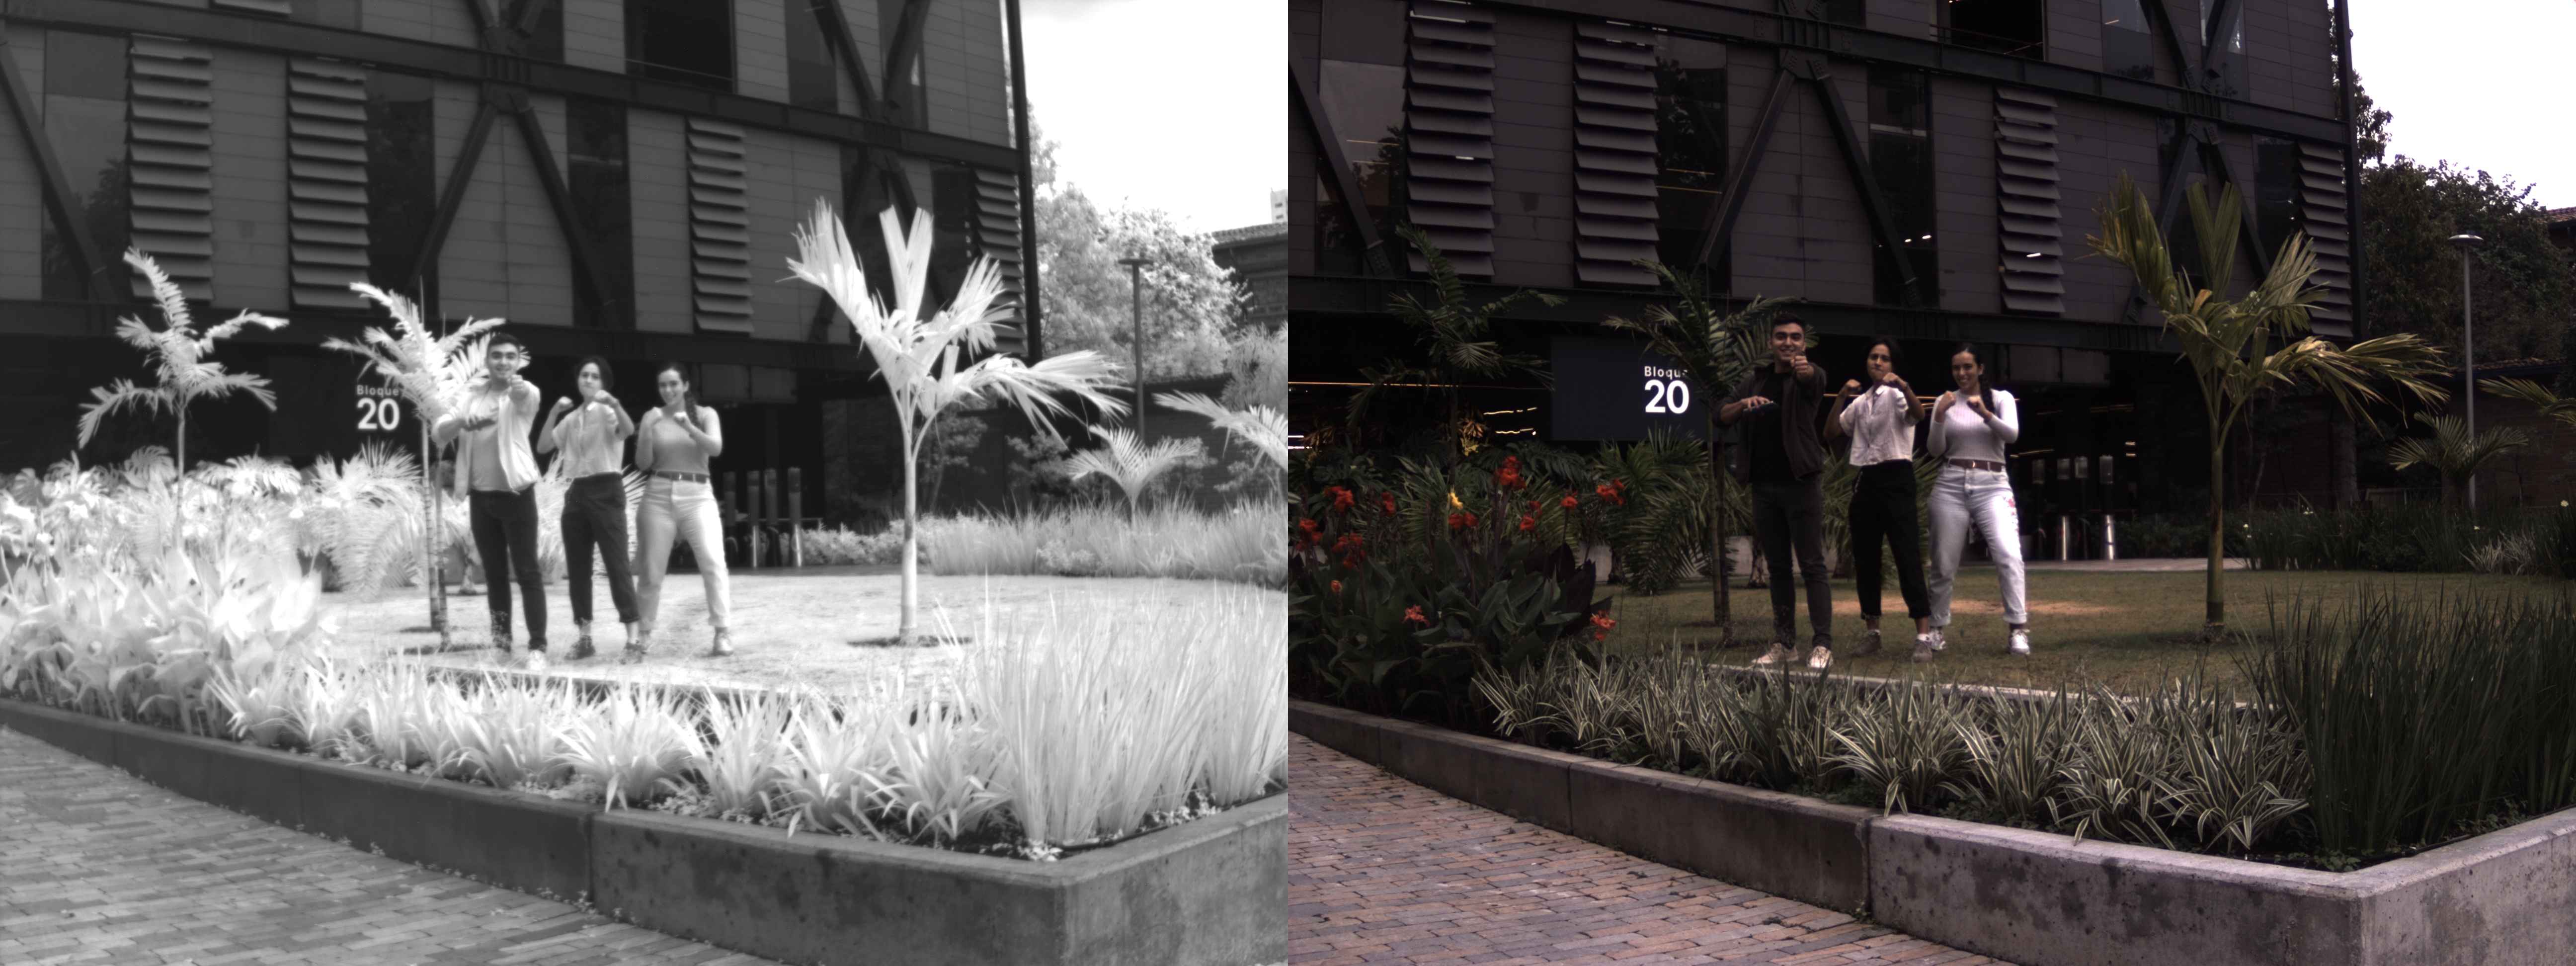
\includegraphics[width=1\textwidth]{Figures/C4/captured_image_20240201_174102.jpg}
        \caption{Captura de imagen realizada durante prueba terrestre mediante control remoto desde un tel'efono inteligente. La imagen muestra la composici'on de ambos canales VIS y NIR, confirmando la funcionalidad del sistema \textit{QBee} en condiciones operativas reales.}
        \label{fig:captura_prueba_remota}
        \end{figure}
        
        \noindent En complemento, en la Figura~\ref{fig:gps_overlay_visual} se presenta un ejemplo de visualización del sistema de coordenadas geográficas en tiempo real. En la parte superior de la imagen se observa la superposición del texto con la latitud, longitud, altitud, velocidad y rumbo extraídos del módulo GPS integrado en la \textit{QBee}. Esta funcionalidad es crítica para asegurar la trazabilidad espacial de las imágenes adquiridas y para su posterior georreferenciación.

        \begin{figure}[h]
            \centering
            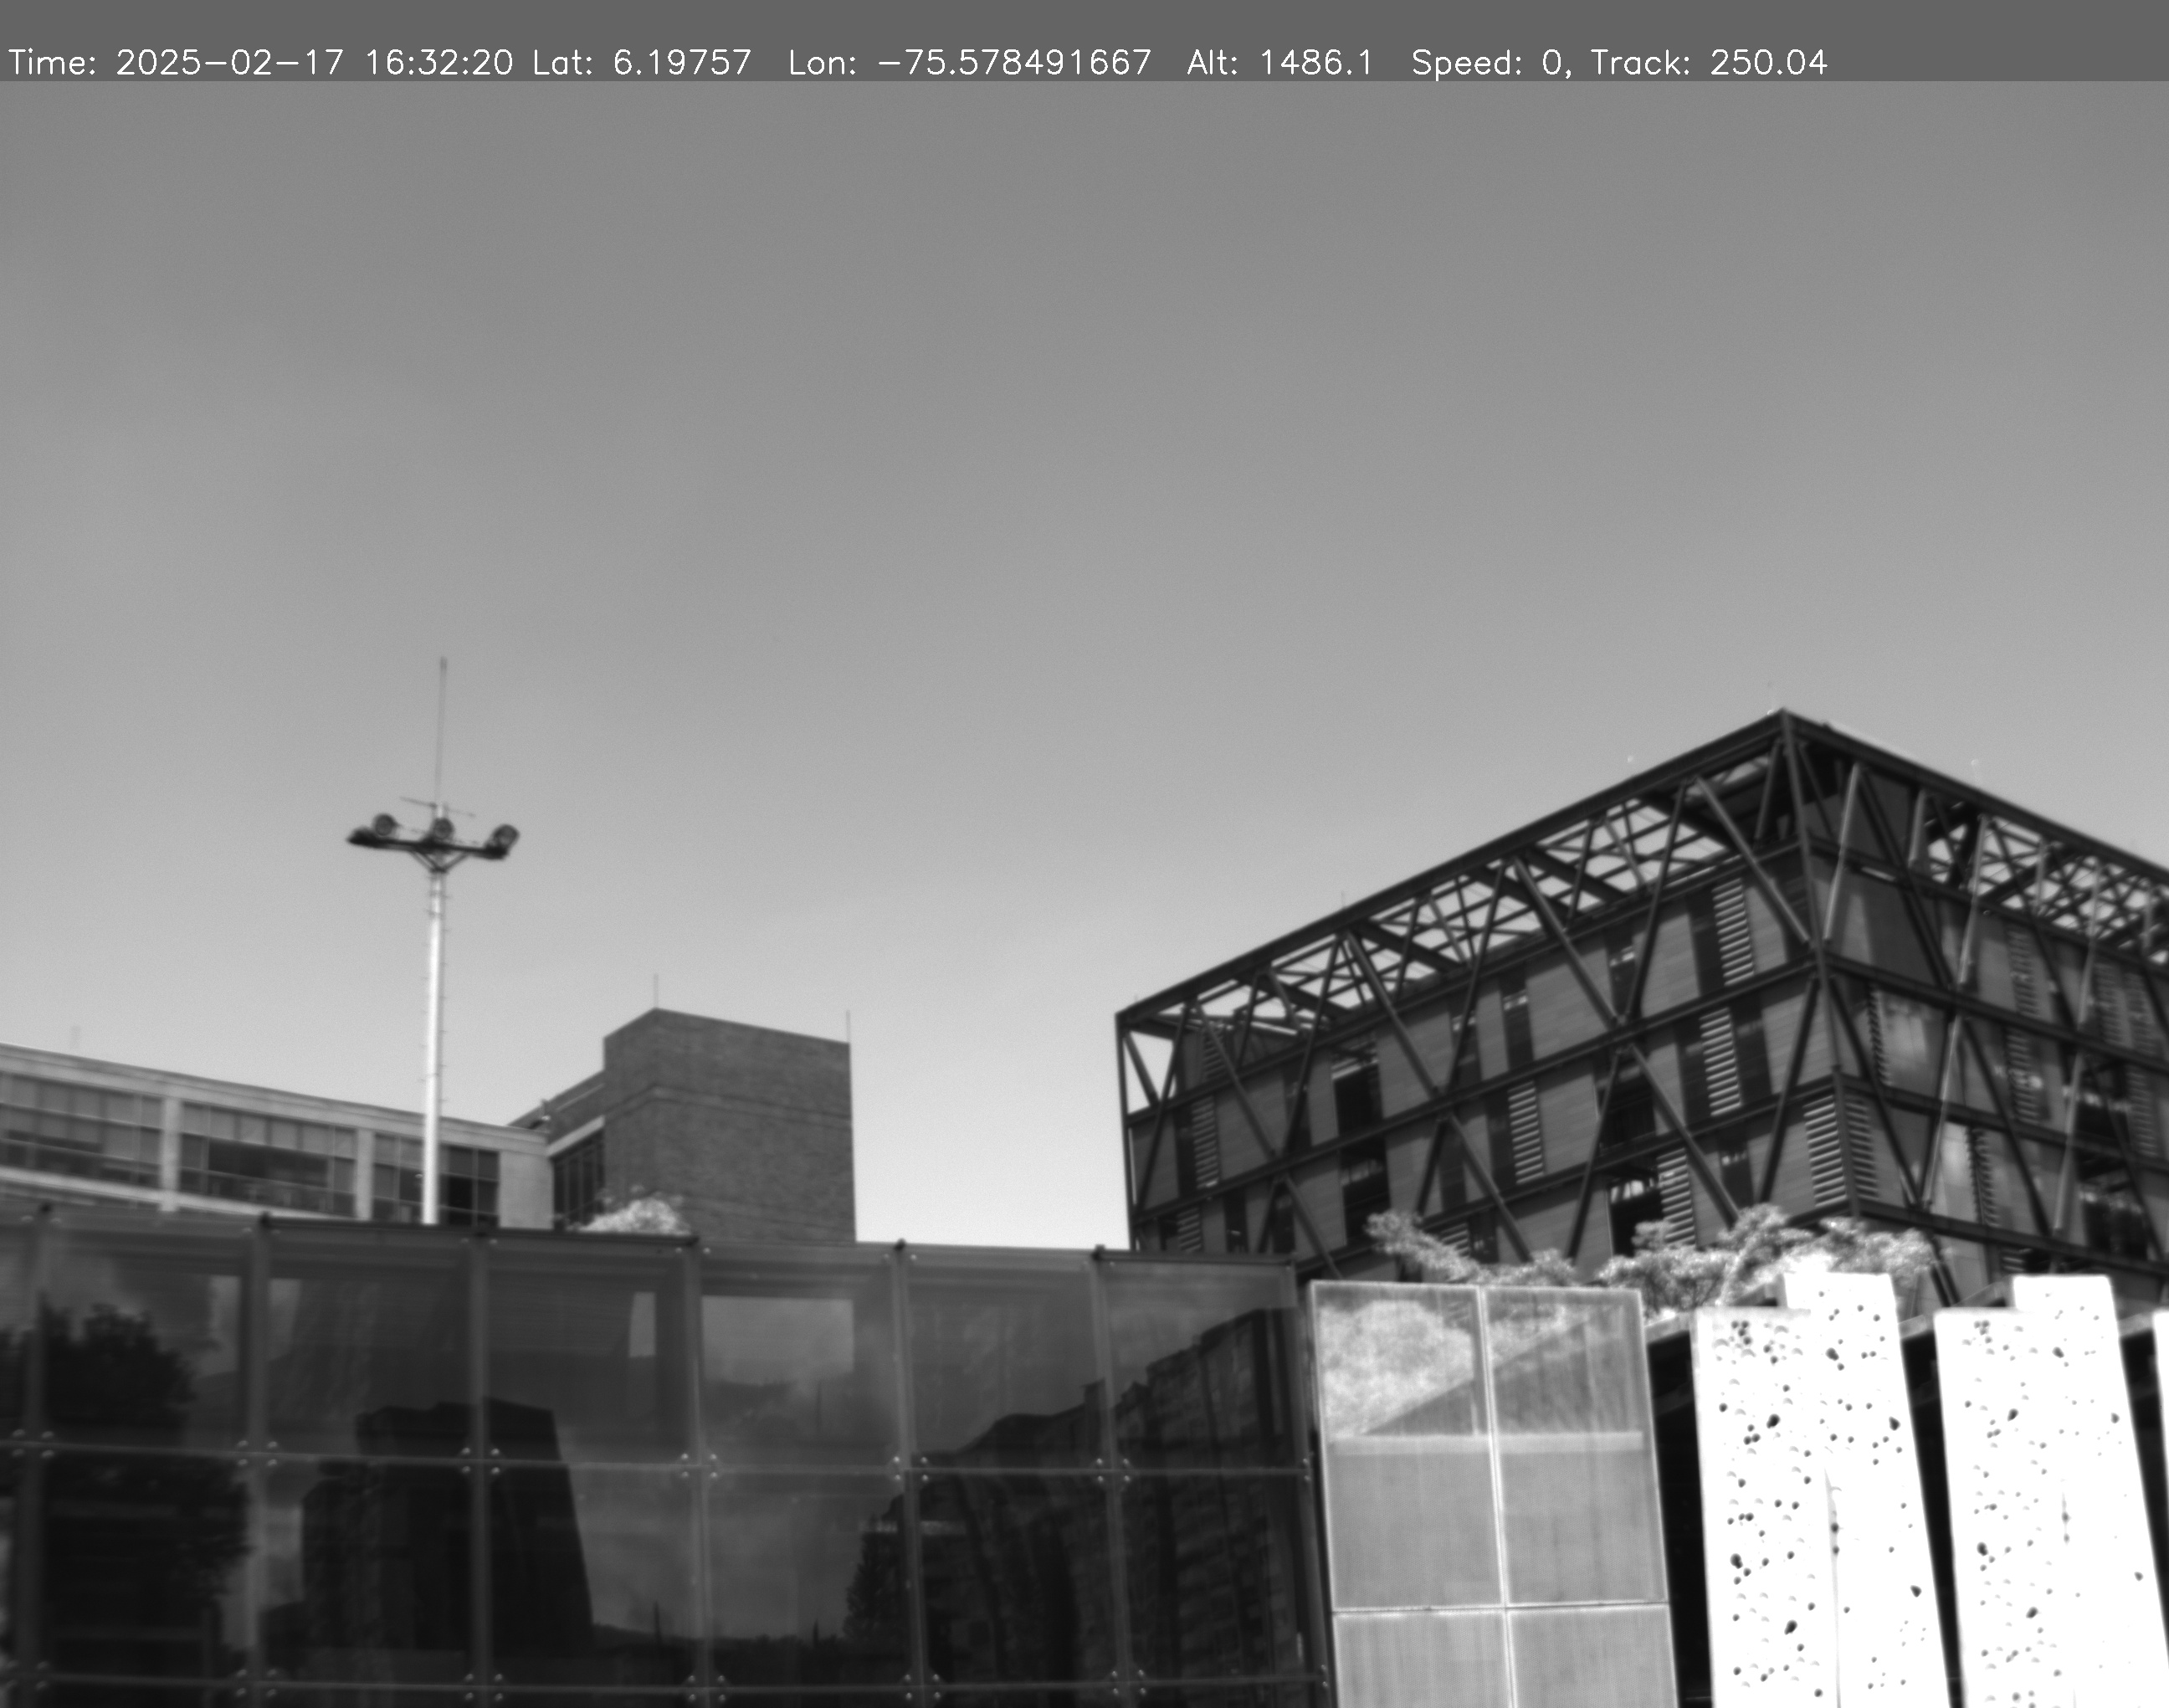
\includegraphics[width=0.9\textwidth]{Figures/C4/captured_image_20250217_113221.jpg}
            \caption{Visualización del sistema de coordenadas geográficas (GPS) en tiempo real sobre la imagen capturada. Se muestran latitud, longitud, altitud, velocidad y rumbo, extraídos automáticamente del módulo GPS durante las pruebas.}
            \label{fig:gps_overlay_visual}
        \end{figure}



    \subsubsection{Pruebas en superficie en condiciones extremas}

    Durante la VII Campa~na A'erea y XI Expedici'on Cient'ifica a la Ant'artida organizada por la Fuerza A'erea Colombiana, el sistema \textit{QBee} fue sometido a una prueba de funcionamiento en condiciones clim'aticas extremas. En este escenario, se enfrent'o a temperaturas diurnas promedio cercanas a los \SI{0}{\celsius}, significativamente inferiores a las condiciones habituales en las cuales opera el sistema.
    
    \noindent El objetivo principal de esta prueba fue evaluar la capacidad del dispositivo para operar de manera confiable en ambientes fr'ios. Se identific'o que, bajo estas condiciones, el sistema present'o fallas intermitentes en su funcionamiento: en algunas ocasiones la \textit{QBee} no inici'o correctamente, o no fue capaz de realizar la grabaci'on de video como lo hace regularmente. Estas fallas pueden estar asociadas a una inicializaci'on deficiente del sistema de procesamiento (Raspberry Pi 4), o a alteraciones en el comportamiento de los sensores VIS y NIR debido a la baja temperatura.
    
    \noindent No obstante, tambi'en se registraron casos exitosos de captura de video, lo cual demuestra que el sistema \textit{QBee} puede llegar a operar de forma funcional en condiciones de fr'io extremo. Estos resultados parciales abren la posibilidad de implementar ajustes de hardware y software para robustecer el funcionamiento del sistema en ambientes m'as hostiles. Queda como trabajo futuro el estudio detallado de las causas espec'ificas de las fallas observadas, as'i como la exploraci'on de soluciones que permitan una operaci'on m'as confiable en entornos como la Ant'artida.
    
    \noindent A pesar de los resultados mixtos, se concluye que el sistema actual no est'a dise~nado para misiones operativas regulares en la Ant'artida u otras regiones con condiciones ambientales similares, sin modificaciones adicionales en aislamiento t'ermico, tolerancia de componentes y procedimientos de inicializaci'on.
    
    \begin{figure}[h]
    \centering
    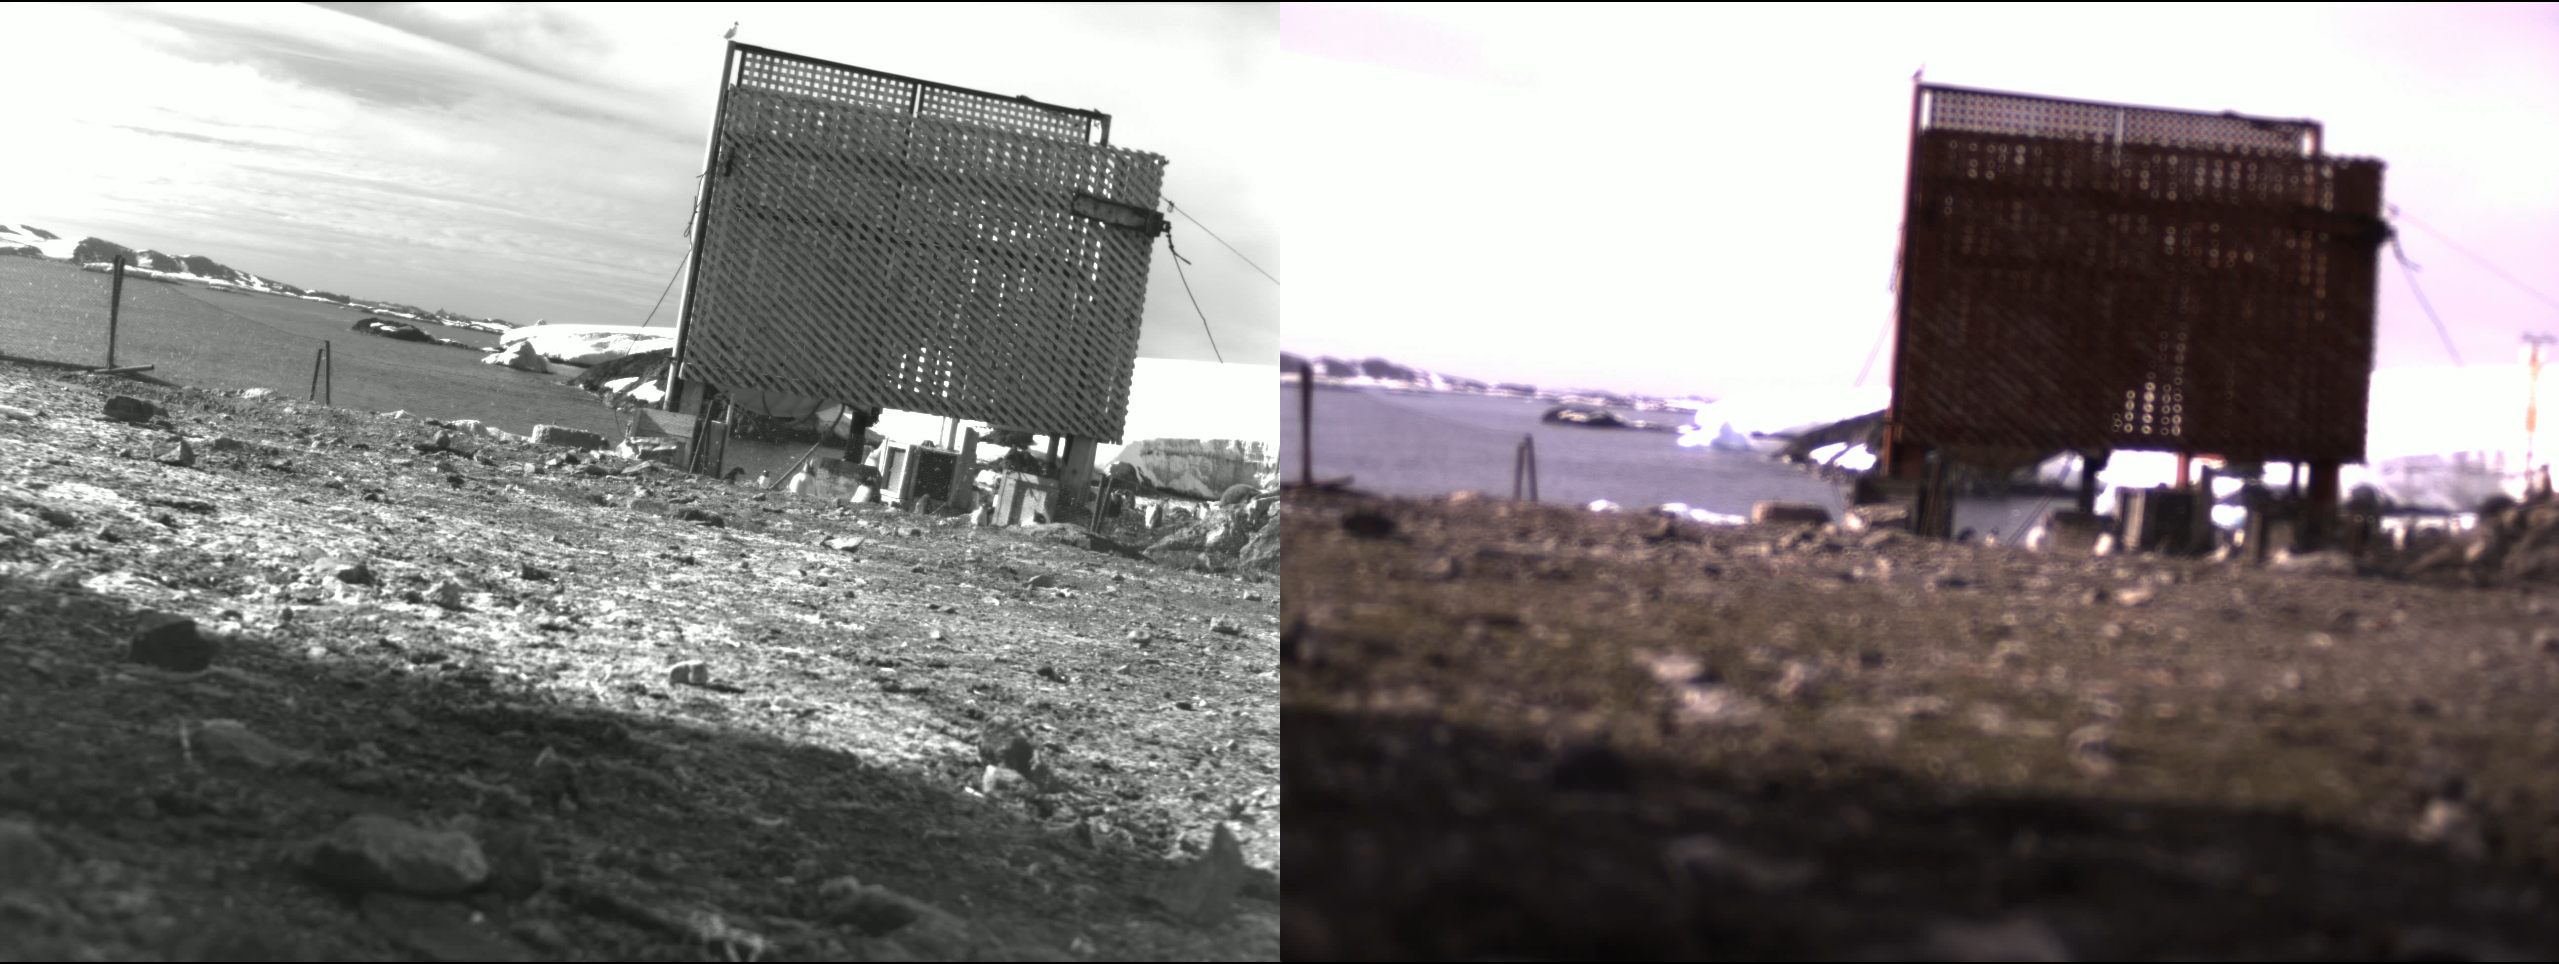
\includegraphics[width=1\textwidth]{Figures/C4/pinguinos.png}
    \caption{Captura de video realizada exitosamente durante la expedición científica en la Antártida. La imagen confirma que, a pesar de las condiciones extremas, el sistema \textit{QBee} En la imagen se aprecia que la cámara visible no se encuentra correctamente enfocada, lo que puede deberse a un mal ajuste de la distancia entre el objetivo y el sensor. Sin embargo, este tipo de desajuste es corregible mediante ajuste mecánico y no afecta el funcionamiento general del sistema \textit{QBee}. fue capaz de operar y registrar datos multiespectrales de forma puntual.}
    \label{fig:prueba_antartida}
    \end{figure}

    \subsubsection{Pruebas en vuelo}

    Las pruebas en vuelo del sistema \textit{QBee} fueron posibles gracias a la colaboraci'on con la Fuerza A'erea Colombiana, la cual facilit'o el montaje del dispositivo en distintas aeronaves de su flota. En una primera prueba, la unidad \textit{QBee} fue instalada a bordo de una aeronave Cessna 208 Caravan, realizando un vuelo a una altitud aproximada de 5000 pies.
    
    \noindent El vuelo se desarroll'o en condiciones ideales, con un rumbo y comportamiento t'ipico de una ruta comercial y sin presencia de perturbaciones atmosf'ericas significativas. Durante toda la duraci'on del trayecto, el sistema oper'o de forma estable y sin presentar inconvenientes.
    
    \noindent Como parte de esta prueba, se verific'o la capacidad de monitoreo remoto del sistema utilizando una red Wi-Fi habilitada dentro de la aeronave, mediante la cual se accedi'o al entorno gr'afico de la Raspberry Pi utilizando el protocolo VNC. Esta conexi'on permiti'o observar en tiempo real la adquisici'on de datos por parte del sistema, confirmando la funcionalidad completa del script y la respuesta de los sensores.
    
    \begin{figure}[!h]
    \centering
    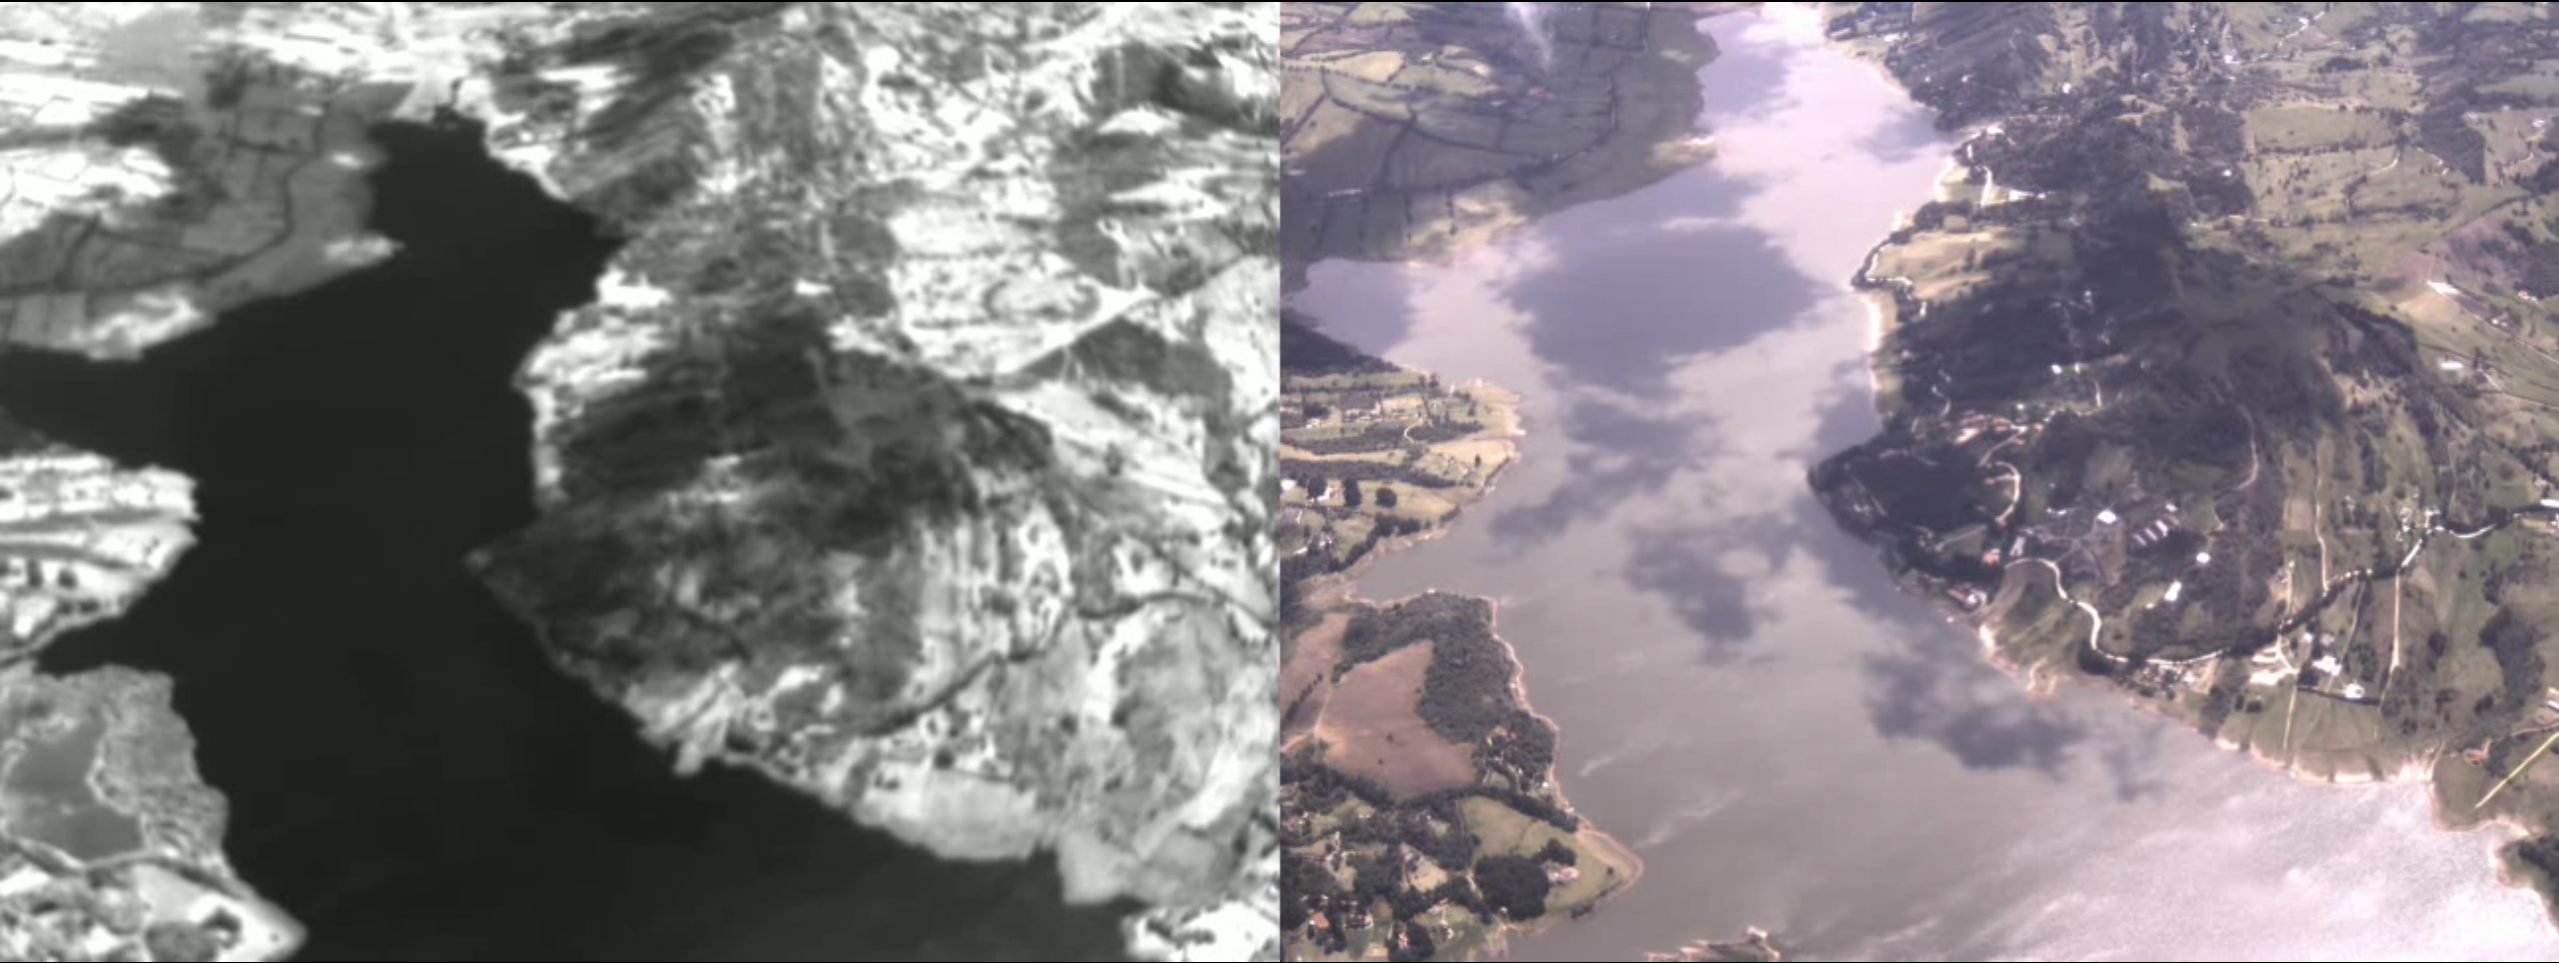
\includegraphics[width=1\textwidth]{Figures/C4/vuelo_caravan.png}
    \caption{Captura tomada durante el vuelo de prueba en la aeronave Cessna 208 Caravan. Se observ'o un comportamiento estable del sistema y transmisi'on remota exitosa mediante protocolo VNC.}
    \label{fig:prueba_vuelo}
    \end{figure}

    \noindent En una segunda prueba, la unidad \textit{QBee} fue montada a bordo de una aeronave de combate Tucano T-27, con el fin de validar su desempeño bajo condiciones de vuelo más exigentes. En este caso, no se contó con un sistema de monitoreo en tiempo real debido a las restricciones propias de la aeronave. Sin embargo, el sistema operó de forma autónoma durante la misión, registrando exitosamente la captura de video.

    \noindent A diferencia del vuelo en la Cessna Caravan, esta prueba presentó una complejidad adicional, ya que durante la operación se ejecutaron maniobras que alcanzaron aceleraciones de hasta 4g. A pesar de estas condiciones dinámicas, la \textit{QBee} logró completar su función de adquisición sin incidentes, lo cual representa un resultado relevante sobre la robustez mecánica y operativa del sistema.
    
    \begin{figure}[!h]
    \centering
    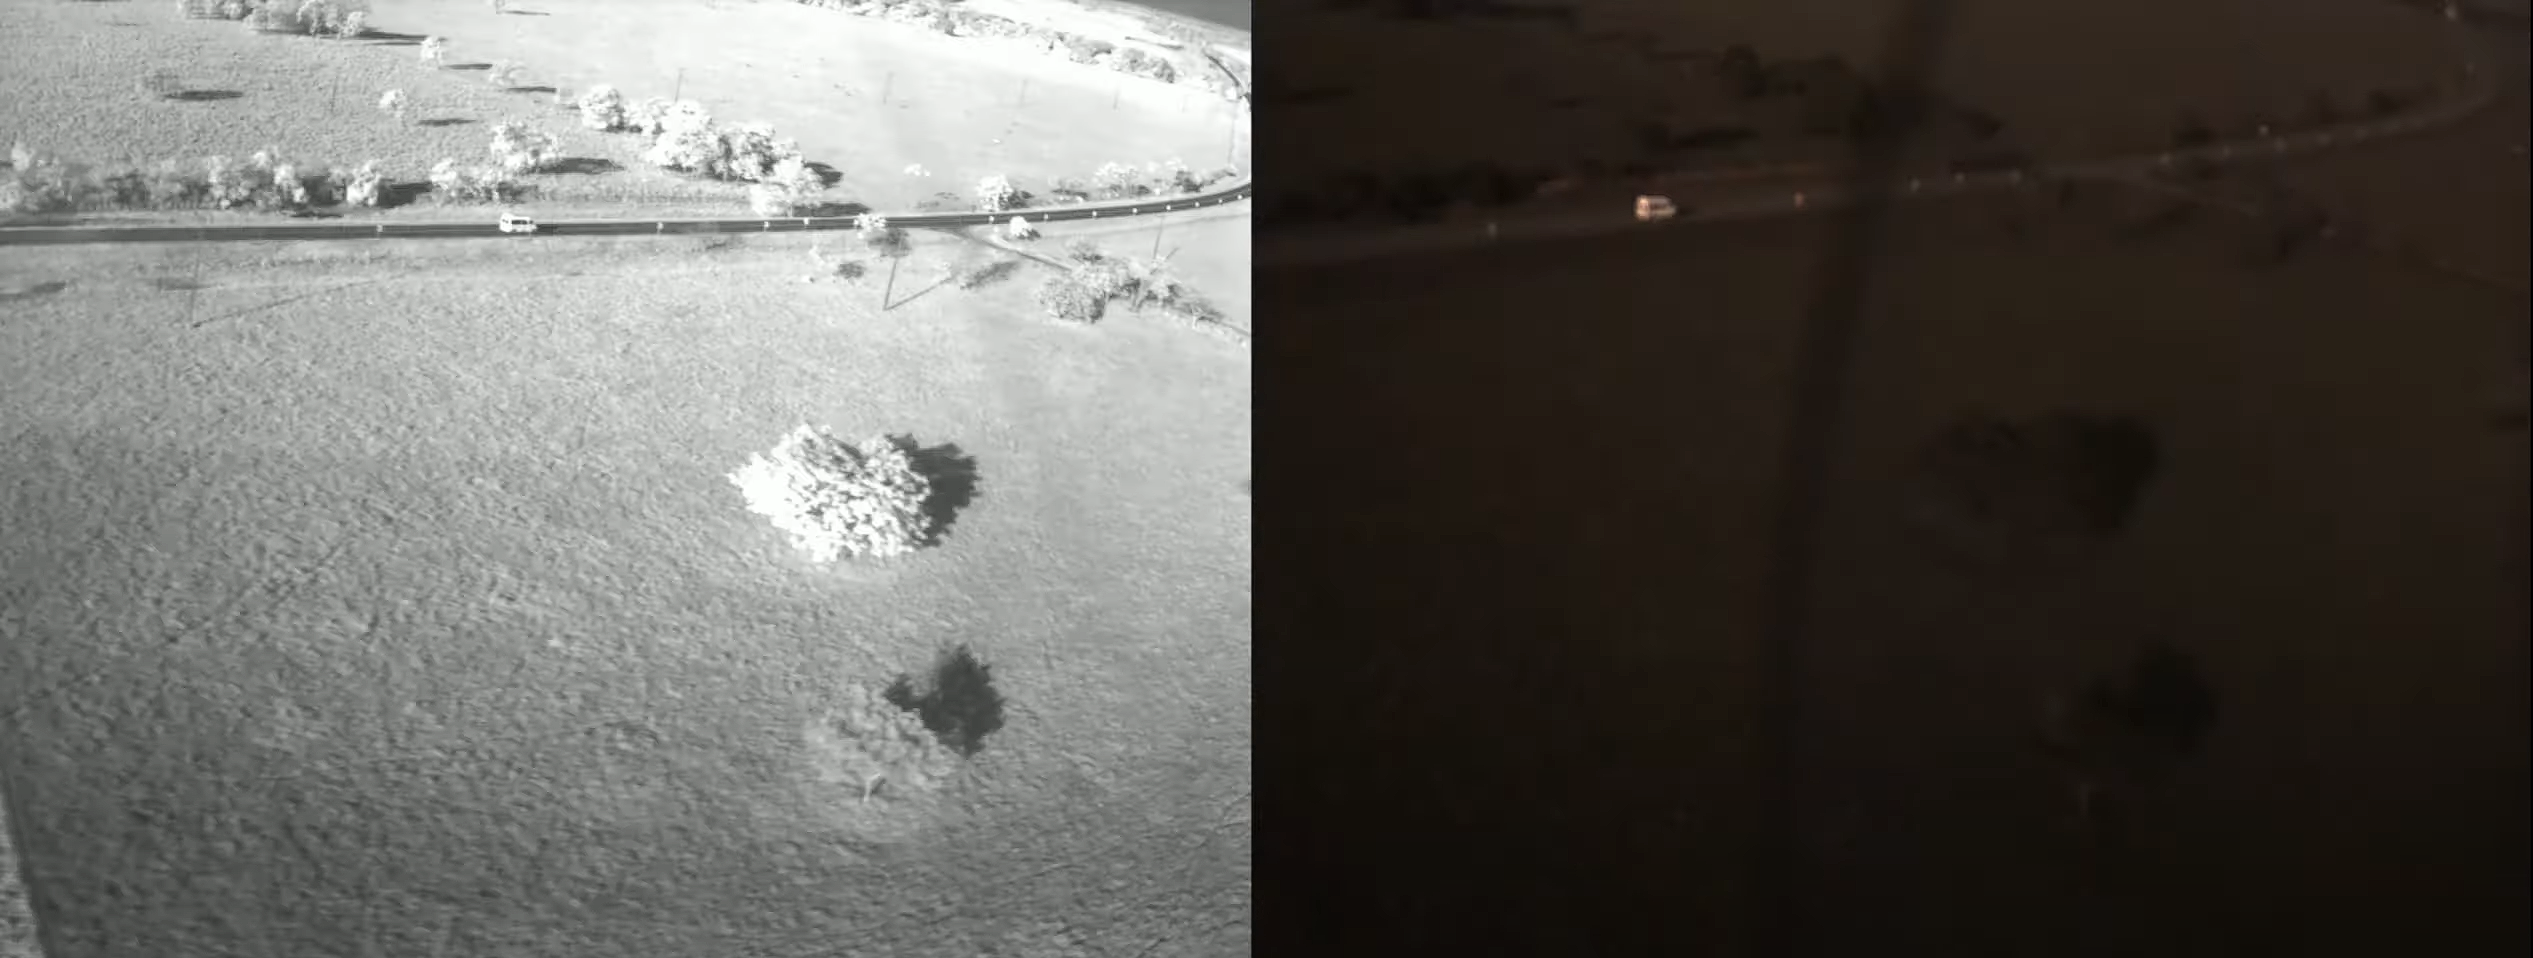
\includegraphics[width=0.9\textwidth]{Figures/C4/t2.png}
    \caption{Captura de video realizada durante prueba a bordo del avión de combate T-27 Tucano. A pesar de las maniobras con aceleraciones de hasta 4g, el sistema \textit{QBee} logró registrar imágenes de forma autónoma y estable. Las condiciones de iluminación ambiental no erán las más adecuadas debido a la hora del día (proximadamente las 6 pm).}
    \label{fig:prueba_tucano}
    \end{figure}

    \section{Conclusiones y lecciones aprendidas}

    temperatura, la saturacion, la cita de velocidad, los links a los videos, sobre el codigo, 